\documentclass[aspectratio=169,11pt]{beamer}

% ---------- Tema semplice, scala di grigi ----------
\usetheme{Boadilla}
\usecolortheme{dove}
\setbeamertemplate{navigation symbols}{}
\setbeamertemplate{caption}{\insertcaption}
\setbeamertemplate{itemize items}[circle]
\setbeamerfont{frametitle}{series=\bfseries}
\setbeamertemplate{frametitle continuation}{}

% ---------- Lingua e codifica ----------
\usepackage[T1]{fontenc}
\usepackage[utf8]{inputenc}
\usepackage[italian]{babel}
\usepackage{graphicx}
\usepackage{booktabs}
\graphicspath{{../relazione/img/}}

% ---------- Colore di accento ----------
\definecolor{whale}{RGB}{0,70,127}
\setbeamercolor{structure}{fg=whale}
\setbeamercolor{frametitle}{fg=whale}

% ---------- Comandi di comodo ----------
\newcommand{\feat}[1]{\texttt{#1}}
\newcommand{\keypoint}[1]{\vspace{0.15cm}\par\footnotesize\textit{#1}}

% ---------- Metadati ----------
\title[Robustezza al rumore]{Studio di robustezza dei modelli di machine learning al rumore nei dati}
\subtitle{Un'analisi sperimentale sul dataset MAGIC Gamma Telescope}
\author[Maccagnan, Bonoli, Chudory]{Daniele Maccagnan \and Matias Bonoli \and Ashley Chudory}
\date{Anno accademico 2025/2026}

\begin{document}

\begin{frame}[plain]
  \titlepage
\end{frame}

\begin{frame}{Indice}
  \tableofcontents
\end{frame}

% ============================================================
\section{Introduzione}
% ============================================================
\begin{frame}{Perché studiare la robustezza al rumore}
  \begin{itemize}
    \item Nei sistemi reali i dati non sono mai perfetti: misure
          imprecise, errori di annotazione, valori mancanti, anomalie, sensori
          guasti.
    \item La domanda non è quale modello sia più accurato sui dati puliti,
          ma quanto ciascuno resiste quando i dati si degradano.
    \item Obiettivo: capire come e perché le prestazioni
          peggiorano in funzione del tipo di disturbo introdotto.
  \end{itemize}
\end{frame}

\begin{frame}{Approccio sperimentale}
  \begin{columns}[t]
    \begin{column}{0.5\textwidth}
      \textbf{Cosa facciamo}
      \begin{itemize}
        \item Calcoliamo una \emph{baseline} sui dati integri.
        \item Corrompiamo il \textbf{solo training set} con sette tipi di rumore.
        \item Tre livelli di intensità crescente: $10\%$, $25\%$, $40\%$.
        \item Riaddestriamo i modelli ad ogni livello.
      \end{itemize}
    \end{column}
    \begin{column}{0.5\textwidth}
      \textbf{Come valutiamo}
      \begin{itemize}
        \item Metriche sempre su un \textbf{test set pulito} e inalterato.
        \item Quattro metriche: accuratezza, F1 macro, recall macro, AUC.
        \item Tre modelli con difese crescenti contro il rumore.
        \item Un esperimento non supervisionato.
      \end{itemize}
    \end{column}
  \end{columns}
  \vfill
  Seme fissato (\texttt{seed = 42}) su tutte le componenti stocastiche per la riproducibilità.
\end{frame}

% ============================================================
\section{Dataset ed esplorazione}
% ============================================================
\begin{frame}{Il dataset MAGIC Gamma Telescope}
  \begin{columns}[c]
    \begin{column}{0.56\textwidth}
      \begin{itemize}
        \item Simulazioni Monte Carlo del telescopio Cherenkov MAGIC.
        \item Ogni record è una  traccia luminosa di un evento atmosferico.
        \item Classificazione binaria: 
              \textbf{gamma (1)} vs \textbf{adroni (0)}.
        \item $19\,020$ osservazioni, $10$ feature continue $+$ target.
      \end{itemize}
    \end{column}
    \begin{column}{0.44\textwidth}
      \centering
      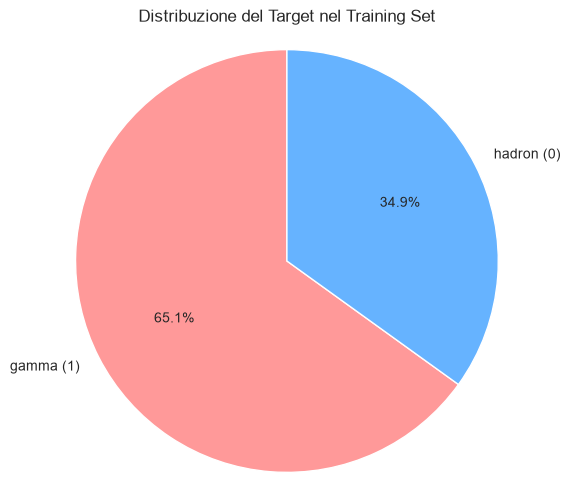
\includegraphics[width=\linewidth]{eda_pie}\\
      {\small Classi sbilanciate: $64{,}8\%$ gamma, $35{,}2\%$ adroni.}
    \end{column}
  \end{columns}
\end{frame}

\begin{frame}{Le dieci feature continue}
  \centering
  \footnotesize
  \begin{tabular}{ll}
    \toprule
    \textbf{Feature} & \textbf{Descrizione} \\
    \midrule
    \feat{fLength}  & lunghezza dell'asse maggiore dell'ellisse \\
    \feat{fWidth}   & lunghezza dell'asse minore dell'ellisse \\
    \feat{fSize}    & logaritmo della somma delle intensità dei pixel \\
    \feat{fConc}    & rapporto di concentrazione dei due pixel più intensi \\
    \feat{fConc1}   & rapporto di concentrazione del pixel più intenso \\
    \feat{fAsym}    & asimmetria della distribuzione lungo l'asse maggiore \\
    \feat{fM3Long}  & momento terzo lungo l'asse maggiore \\
    \feat{fM3Trans} & momento terzo lungo l'asse minore \\
    \feat{fAlpha}   & angolo tra asse maggiore e direzione del centro campo \\
    \feat{fDist}    & distanza dal centro del campo all'origine dell'ellisse \\
    \bottomrule
  \end{tabular}
  \keypoint{Le feature codificano \textbf{geometria} e \textbf{distribuzione di
  intensità} dell'immagine.}
\end{frame}

\begin{frame}{Suddivisione dei dati}
  \textbf{Split stratificato $60/20/20$}
    \begin{itemize}
        \item $11\,412$ train, $3\,804$ val, $3\,804$ test.
        \item Split \emph{prima} di ogni analisi: niente \textbf{data leakage}.
        \item Stratificazione sul target: ogni partizione conserva il rapporto
              gamma/adroni.
      \end{itemize}
  \vfill
  EDA condotta solo sul training
\end{frame}

\begin{frame}{EDA: Distribuzioni delle feature}
  \centering
  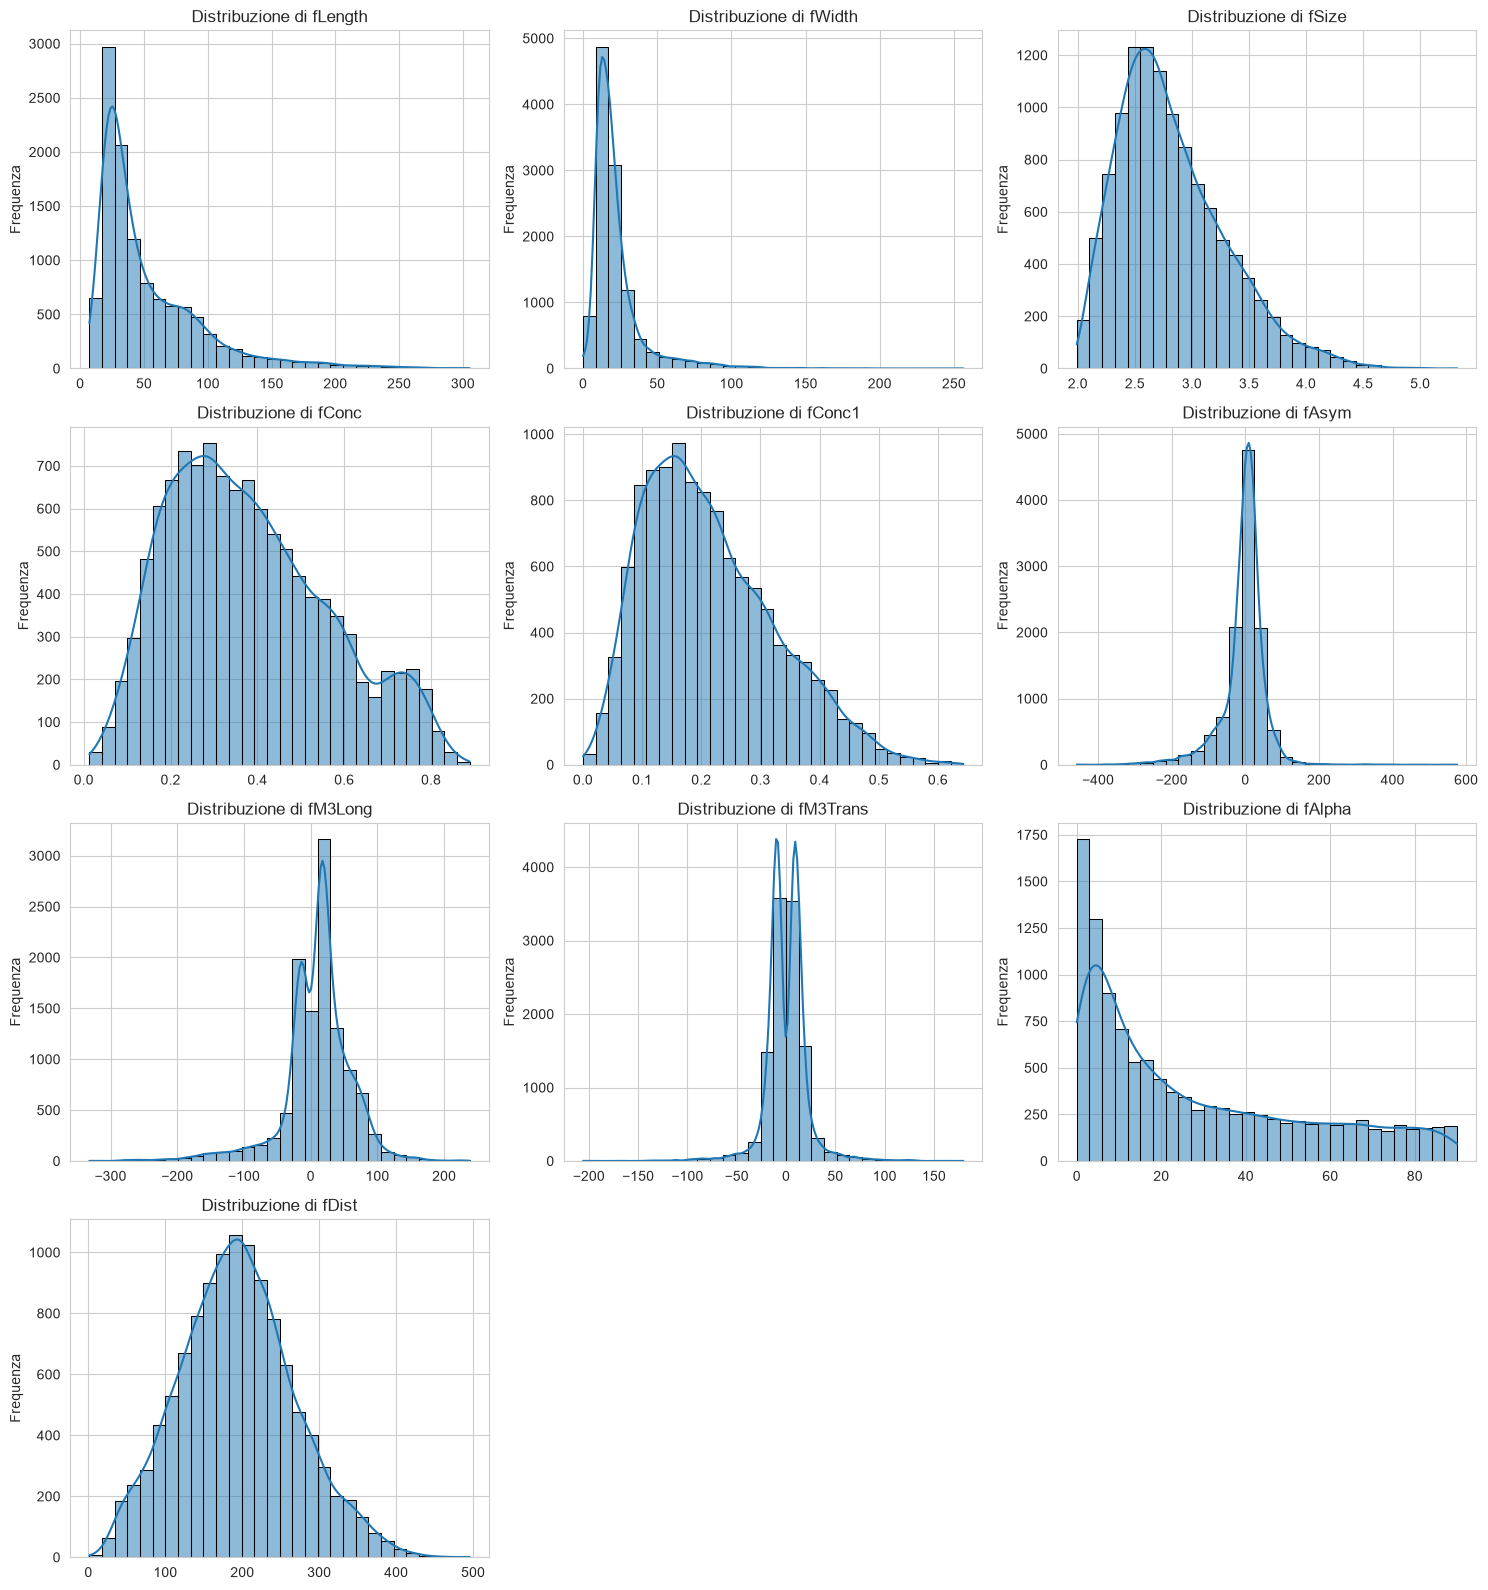
\includegraphics[height=0.70\textheight]{eda_hist}\\
  {\small Distribuzioni \textbf{asimmetriche}, code lunghe e
  scale eterogenee da unità a centinaia.}
\end{frame}

\begin{frame}{EDA: boxplot per classe}
  \centering
  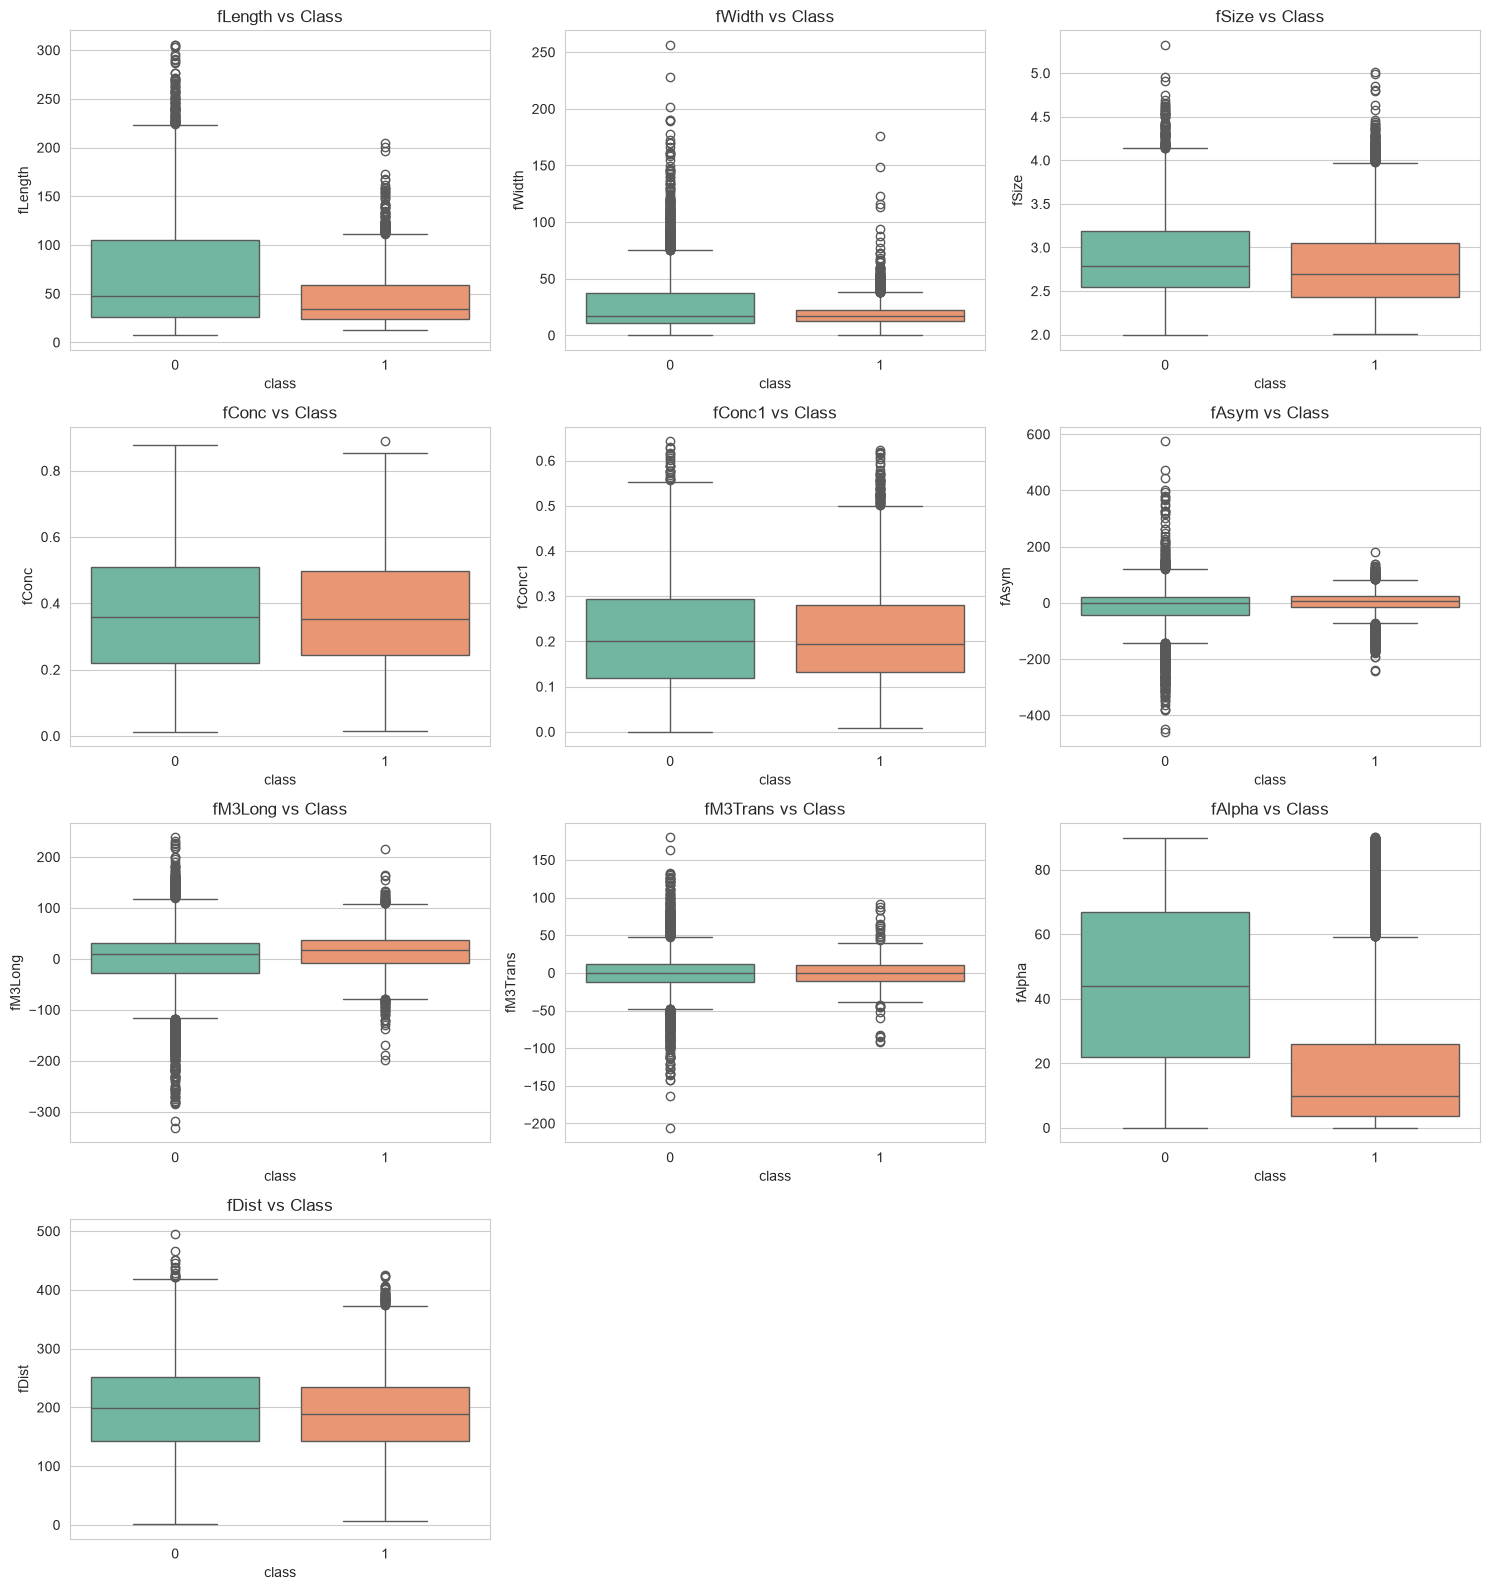
\includegraphics[height=0.70\textheight]{eda_box}\\
  {\small \feat{fAlpha} è la più discriminante; seguono \feat{fLength},
  \feat{fWidth}, \feat{fSize}. Le restanti feature separano meno le classi.}
\end{frame}

\begin{frame}{EDA: Correlazioni}
  \begin{columns}[c]
    \begin{column}{0.58\textwidth}
      \centering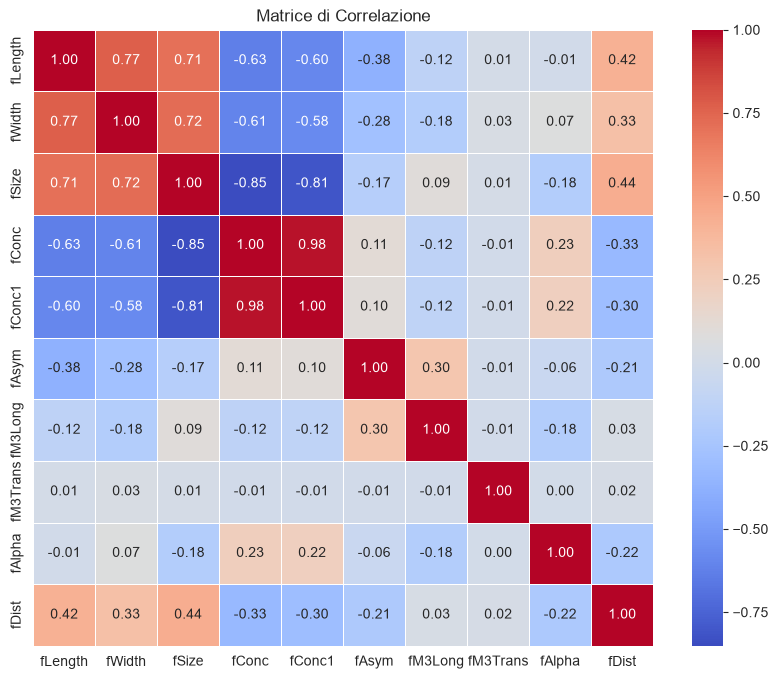
\includegraphics[width=\linewidth]{eda_corr}
    \end{column}
    \begin{column}{0.42\textwidth}
      \begin{itemize}
        \item \feat{fConc}/\feat{fConc1} quasi ridondanti ($0{,}98$).
        \item Anticorrelazione con \feat{fSize} ($-0{,}85$).
        \item \feat{fLength}/\feat{fWidth}/\feat{fSize} correlate
              ($0{,}70$--$0{,}77$).
        \item Vi è ridondanza di informazione: il disturbo su una feature è in
              parte compensato dalle altre.
        \item \feat{fAlpha} quasi scorrelata: informazione unica e non
              sostituibile.
      \end{itemize}
    \end{column}
  \end{columns}
\end{frame}

\begin{frame}{Preprocessing}
  \textbf{Standardizzazione}
    \begin{itemize}
      \item Normalizzazione del dataset: media $0$, deviazione standard $1$.
      \item Parametri stimati \textbf{solo sul training}, applicati a val/test: no data leakage.
      \item Essenziale per la convergenza delle reti neurali.
    \end{itemize}
  \end{frame}

% ============================================================
\section{Modelli e baseline}
% ============================================================
\begin{frame}{I tre modelli}
  \begin{itemize}
    \item \textbf{NN Base} -- Rete neurale semplice: Dense(32)$\to$Dense(16)$\to$
          sigmoide. Nessuna regolarizzazione, Adam $10^{-3}$, $75$ epoche.
          Libero di andare in overfitting.
    \item \textbf{NN Pro} -- stessa architettura $+$ quattro difese:
          \begin{itemize}
            \item[$\circ$] regolarizzazione \emph{L2} ($10^{-4}$);
            \item[$\circ$] \emph{dropout} ($0{,}2$);
            \item[$\circ$] \emph{class weight} bilanciato a favore degli adroni;
            \item[$\circ$] \emph{early stopping} sulla validation loss con patience $15$.
          \end{itemize}
    \item \textbf{Random Forest} -- $200$ alberi, bagging e voto di
          maggioranza: la varianza degli errori individuali si cancella.
  \end{itemize}
  \vfill
  Quattro metriche di valutazione principali: accuratezza, F1
  macro, recall macro, AUC. Le macro pesano ugualmente le due classi.
\end{frame}
  


\begin{frame}{Baseline su dati puliti}
  \begin{columns}[c]
    \begin{column}{0.52\textwidth}
      \centering
      \footnotesize
      \begin{tabular}{lccc}
        \toprule
        & Acc & F1$_m$ & AUC \\
        \midrule
        NN Base & 0,8678 & 0,8517 & 0,9214 \\
        NN Pro  & 0,8601 & 0,8468 & 0,9238 \\
        RF      & \textbf{0,8785} & \textbf{0,8629} & \textbf{0,9300} \\
        \bottomrule
      \end{tabular}
      \vspace{0.4cm}
      \begin{itemize}
        \item Modelli quasi equivalenti, tutti ben oltre la soglia banale
              del $65\%$.
        \item \textbf{RF} il migliore su tutte le metriche.
        \item NN Pro cede accuratezza (class weight) ma ha \textbf{AUC più alta}
              della rete Base.
      \end{itemize}
    \end{column}
    \begin{column}{0.44\textwidth}
      \centering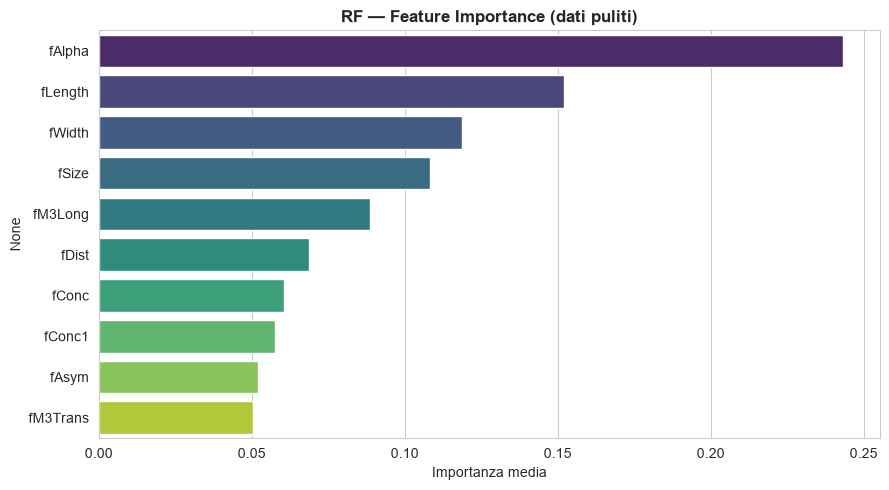
\includegraphics[width=\linewidth]{baseline_featimp}\\
      {\small \feat{fAlpha} domina la \emph{feature importance} ($\approx 0{,}24$),
      coerente con i boxplot.}
    \end{column}
  \end{columns}
\end{frame}

\begin{frame}{Baseline: matrici di confusione}
  \centering
  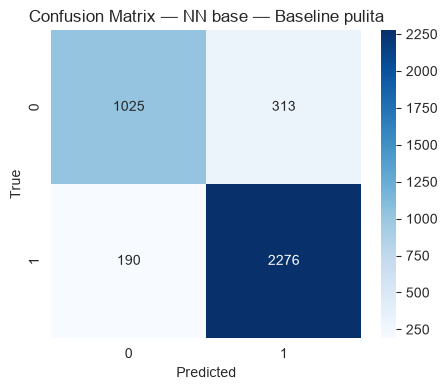
\includegraphics[height=4.3cm]{baseline_nnbase_cm}\hfill
  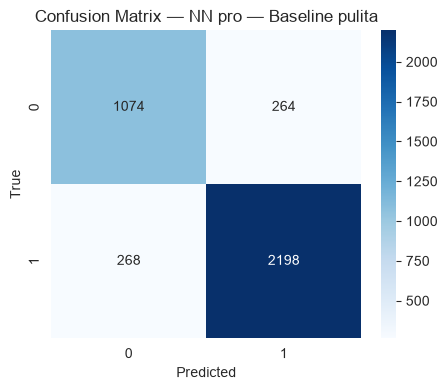
\includegraphics[height=4.3cm]{baseline_nnpro_cm}\hfill
  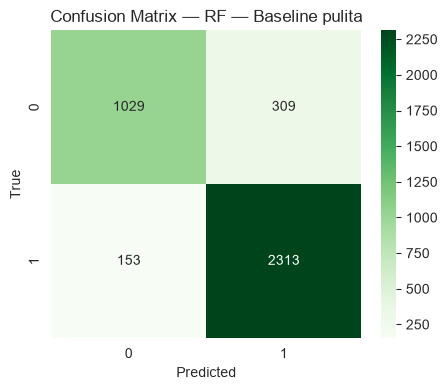
\includegraphics[height=4.3cm]{baseline_rf_cm}\\
  {\scriptsize NN Base, NN Pro, Random Forest.}
  \vfill
  \begin{minipage}{0.9\linewidth}
    \centering
    Tutti riconoscono bene i gamma; gli errori si concentrano sugli
    \textbf{adroni}.
  \end{minipage}
\end{frame}

\begin{frame}{Baseline: curva di addestramento}
  \centering
  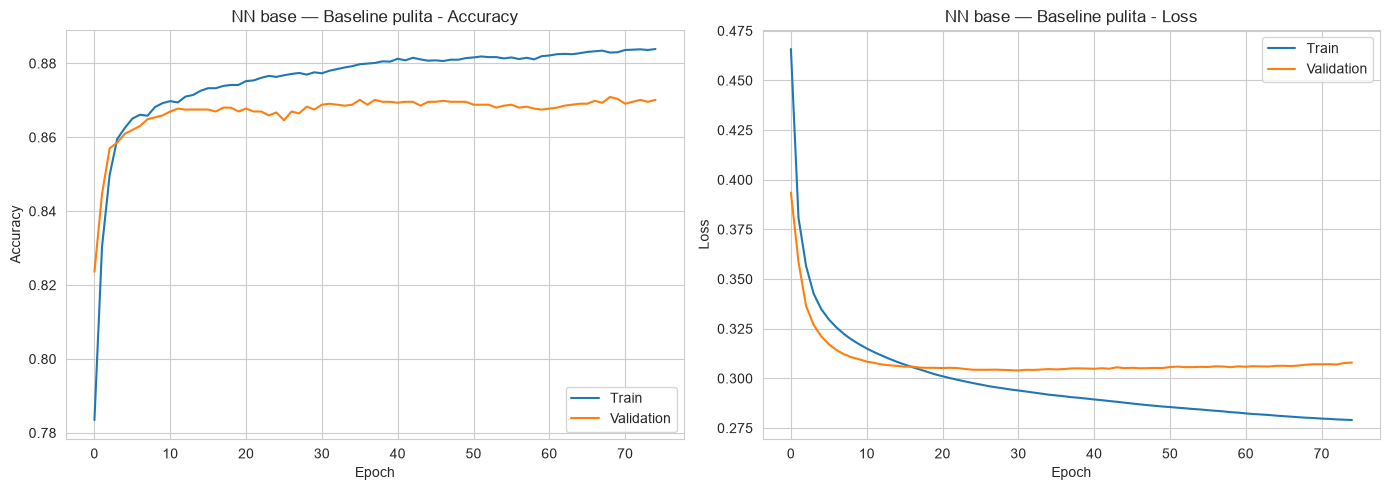
\includegraphics[width=0.85\linewidth]{baseline_nnbase_curve}\\
  {\scriptsize Curva NN Base: convergenza regolare, gap train / validation
  contenuto -- nessun overfitting marcato.}
\end{frame}

% ============================================================
\section{Metodologia del rumore}
% ============================================================
\begin{frame}{Come iniettiamo il rumore}
  \begin{itemize}
    \item Il rumore altera \textbf{solo il training set}; validation e test
          restano puliti $\Rightarrow$ valutiamo la vera generalizzazione.
    \item Per ogni rumore: riaddestramento ai tre livelli ($10\%$, $25\%$, $40\%$)
          e valutazione sullo stesso test set.
    \item Iniezione sul training \emph{già standardizzato}: per perturbazioni
          additive o monotone equivale a corrompere i dati originali.
  \end{itemize}
  \vfill
\end{frame}

\begin{frame}{I sette meccanismi di rumore}
  \footnotesize
  \begin{enumerate}
    \item \textbf{Feature noise}: rumore gaussiano $N(0,\sigma)$ aggiunto a tutte
          le feature con $\sigma$ proporzionale al livello.
    \item \textbf{Feature noise localizzato}: $\sigma=0{,}35$ fisso, ma su un
          numero crescente di feature importanti (top-1 / top-3 / top-5).
    \item \textbf{Label noise random}: etichette invertite a caso.
    \item \textbf{Label noise borderline}: etichette invertite sui campioni
         ambigui vicini al centroidi tra le classi.
    \item \textbf{Missing values}: celle mancanti (\texttt{NaN}) da imputare
          con media o mediana.
    \item \textbf{Outlier}: righe a $\pm 5$ deviazioni standard, segno casuale
          (strategie: nessuna / winsorizzazione / imputazione).
    \item \textbf{Missing feature}: intere colonne azzerate,
          su tutti i set, per importanza decrescente.
  \end{enumerate}
\end{frame}

\begin{frame}{L'effetto dei disturbi su una feature}
  \centering
  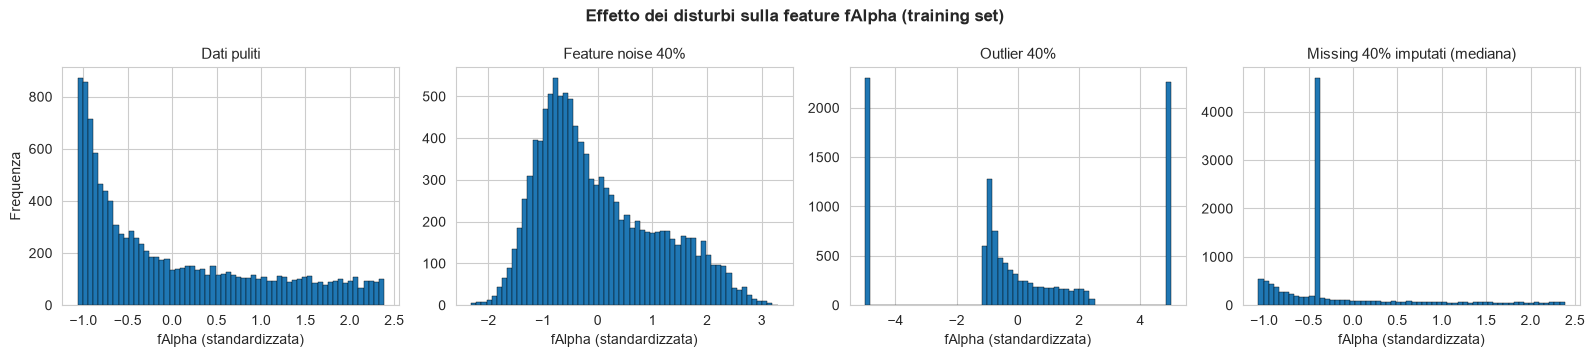
\includegraphics[width=0.95\textwidth]{metodo_falpha}\\
  \vspace{0.15cm}
  {\small \feat{fAlpha} standardizzata: dati puliti e tre disturbi al $40\%$.
  Il rumore gaussiano allarga la distribuzione, gli outlier creano due picchi
  agli estremi, l'imputazione concentra molti campioni su un unico valore.}
\end{frame}

% ============================================================
\section{Risultati per tipo di rumore}
% ============================================================

% ---------- Feature noise ----------
\begin{frame}{Feature noise: analisi}
  \begin{itemize}
    \item Degrado \textbf{graduale}: al $40\%$ tutti i modelli
          restano sopra l'$83\%$ (calo di $3$--$4$ punti).
    \item Al $40\%$ vince la \textbf{NN Pro} ($0{,}8417$): L2 $+$ dropout
          impediscono di apprendere le fluttuazioni casuali.
    \item La NN Base, senza vincoli, si adatta al rumore e peggiora
          sui campioni nuovi.
    \item Degrado \textbf{asimmetrico}: la recall adroni della Base crolla
          $0{,}77 \to 0{,}59$, mentre quella dei gamma sale $0{,}92 \to 0{,}97$.
    \item Il class weight della Pro sostiene la recall degli adroni a $0{,}73$.
  \end{itemize}
  \vfill
\end{frame}

\begin{frame}{Feature noise: metriche e matrici di confusione}
  \centering
  \footnotesize
  \begin{tabular}{c *{9}{c}}
    \toprule
     & \multicolumn{3}{c}{NN Base} & \multicolumn{3}{c}{NN Pro} & \multicolumn{3}{c}{Random Forest}\\
    \cmidrule(lr){2-4}\cmidrule(lr){5-7}\cmidrule(lr){8-10}
    Rumore & Acc & F1$_m$ & AUC & Acc & F1$_m$ & AUC & Acc & F1$_m$ & AUC \\
    \midrule
    Pulito & 0,8678 & 0,85 & 0,9214 & 0,8601 & 0,85 & 0,9238 & 0,8785 & 0,86 & 0,9300 \\
    10\% & 0,8657 & 0,85 & 0,9187 & 0,8636 & 0,85 & 0,9204 & 0,8646 & 0,84 & 0,9222 \\
    25\% & 0,8520 & 0,83 & 0,9074 & 0,8465 & 0,83 & 0,9071 & 0,8494 & 0,82 & 0,9041 \\
    40\% & 0,8328 & 0,80 & 0,8941 & \textbf{0,8417} & \textbf{0,82} & 0,8940 & 0,8318 & 0,80 & 0,8913 \\
    \bottomrule
  \end{tabular}
  \vspace{0.3cm}
  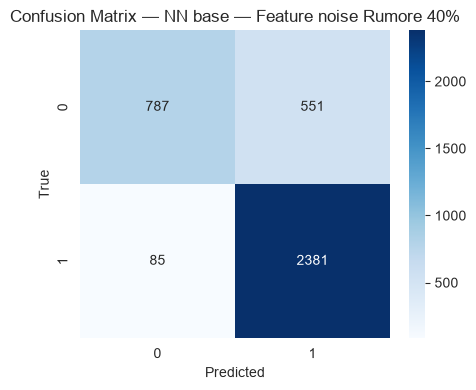
\includegraphics[height=3.9cm]{fn_nnbase_cm40}\hfill
  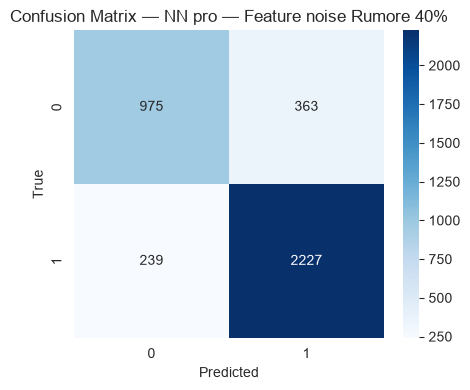
\includegraphics[height=3.9cm]{fn_nnpro_cm40}\hfill
  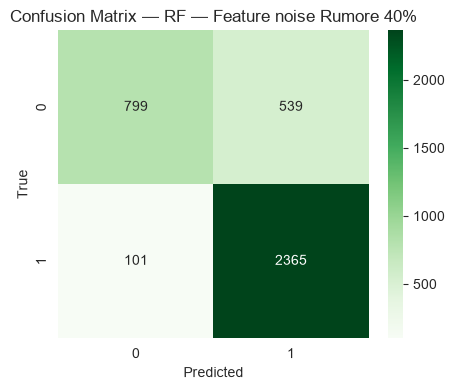
\includegraphics[height=3.9cm]{fn_rf_cm40}\\
  {\scriptsize Matrici di confusione al $40\%$: NN Base, NN Pro, Random Forest.}
\end{frame}

\begin{frame}{Feature noise: curve di addestramento}
  \centering
  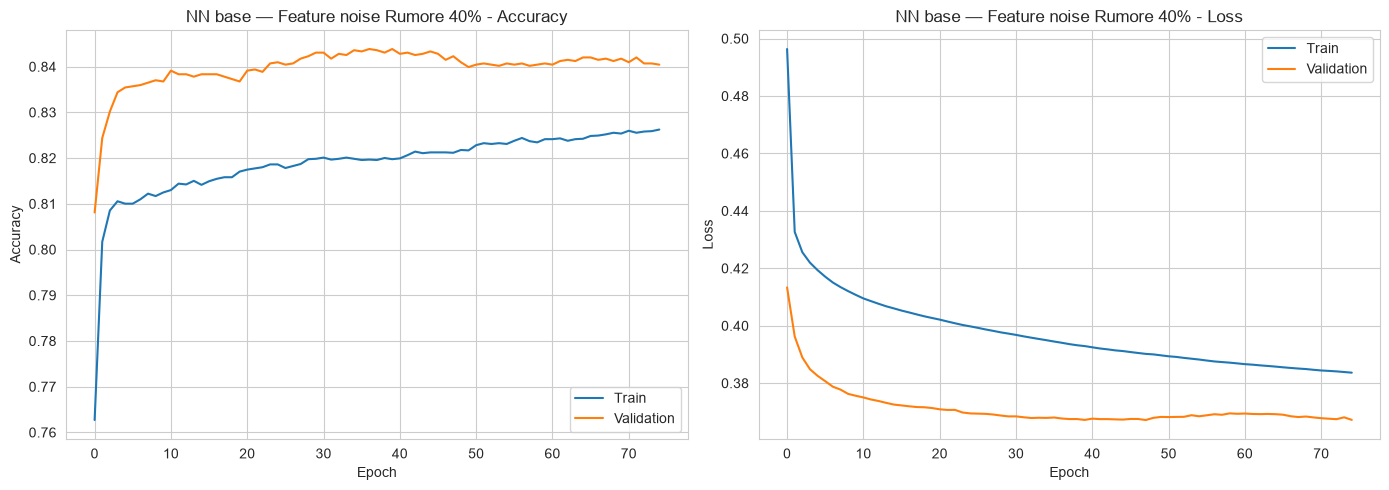
\includegraphics[height=3.3cm]{fn_nnbase_curve40}\hfill
  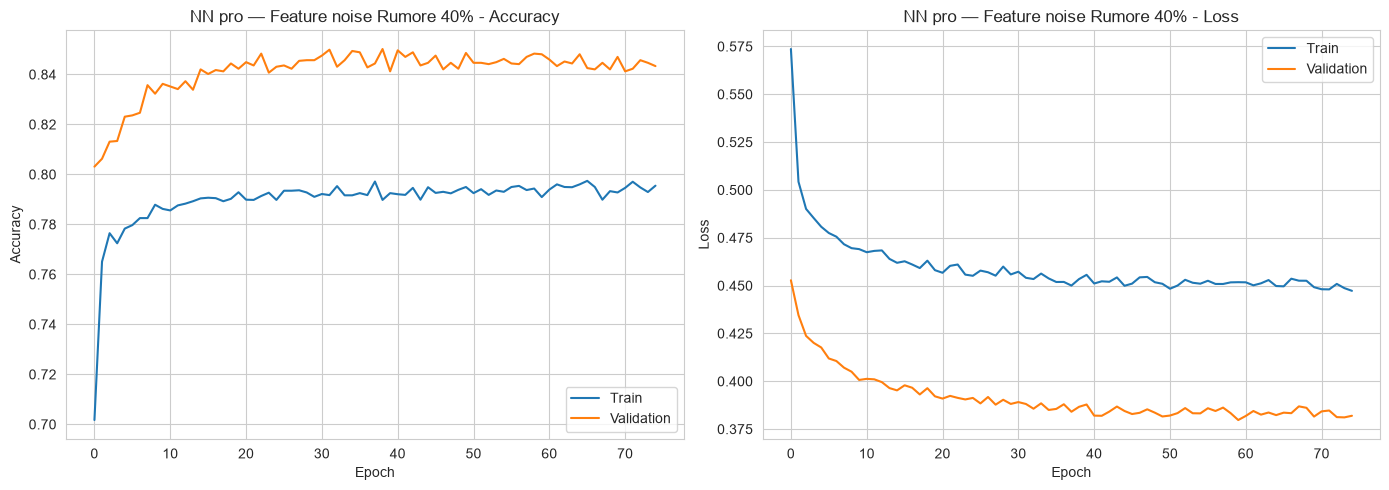
\includegraphics[height=3.3cm]{fn_nnpro_curve40}\\
  {\scriptsize Curve al $40\%$: NN Base (sinistra) vs NN Pro (destra).
  La Pro mantiene train e validation più vicine: L2 e dropout limitano
  l'adattamento al rumore.}
\end{frame}

\begin{frame}{Feature noise: evidenze grafiche}
  \begin{columns}[c]
    \begin{column}{0.5\textwidth}
      \centering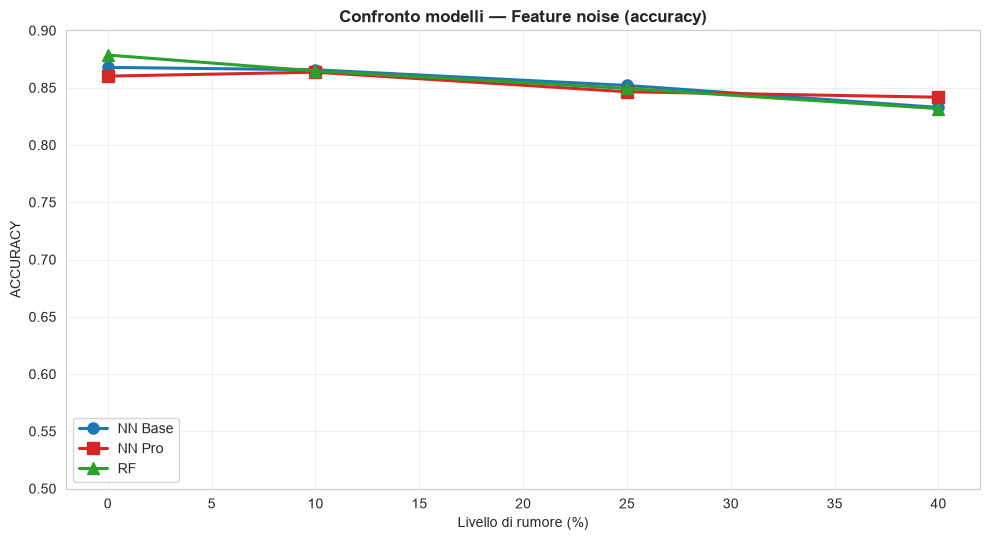
\includegraphics[height=4.0cm]{fn_compare_acc}\\
    \end{column}
    \begin{column}{0.5\textwidth}
      \centering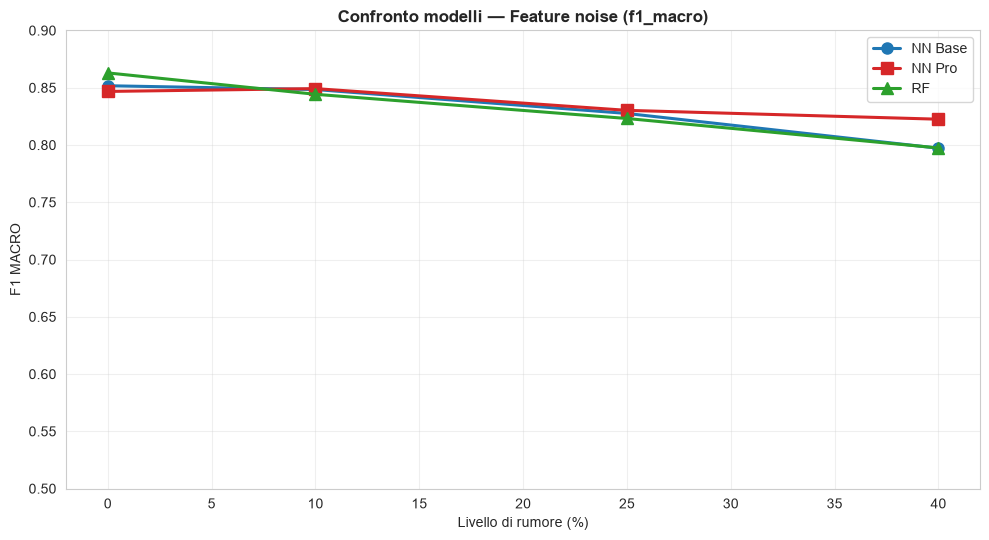
\includegraphics[height=4.0cm]{fn_compare_f1.png}\\
    \end{column}
  \end{columns}
\end{frame}

% ---------- Feature noise localizzato ----------
\begin{frame}{Feature noise localizzato -- analisi}
  \begin{itemize}
    \item Intensità fissa ($\sigma=0{,}35$), ma colpisce solo le feature più
          importanti: top-1 (\feat{fAlpha}) $\to$ top-3 $\to$ top-5.
    \item Degrado comunque \textbf{lieve}: al $40\%$ tutti sopra l'$83\%$.
    \item Stessa asimmetria: recall adroni Base a $0{,}67$, Pro a $0{,}75$.
    \item \textbf{Contrasto chiave con il missing feature:}
          \begin{itemize}
            \item[$\circ$] \emph{disturbare} \feat{fAlpha} $\Rightarrow$ NN Base a
                  $0{,}8651$;
            \item[$\circ$] \emph{azzerarla} $\Rightarrow$ crollo a $0{,}8215$.
          \end{itemize}
  \end{itemize}
  \vfill
  \keypoint{Il rumore \textbf{degrada} l'informazione ma non la cancella:
  un'informazione rumorosa ma presente resta utilizzabile.}
\end{frame}

\begin{frame}{Feature noise localizzato: metriche e matrici di confusione}
  \centering
  \footnotesize
  \begin{tabular}{c *{9}{c}}
    \toprule
     & \multicolumn{3}{c}{NN Base} & \multicolumn{3}{c}{NN Pro} & \multicolumn{3}{c}{Random Forest}\\
    \cmidrule(lr){2-4}\cmidrule(lr){5-7}\cmidrule(lr){8-10}
    Rumore & Acc & F1$_m$ & AUC & Acc & F1$_m$ & AUC & Acc & F1$_m$ & AUC \\
    \midrule
    Pulito & 0,8678 & 0,85 & 0,9214 & 0,8601 & 0,85 & 0,9238 & 0,8785 & 0,86 & 0,9300 \\
    10\% & 0,8651 & 0,85 & 0,9211 & 0,8651 & 0,85 & 0,9243 & 0,8743 & 0,86 & 0,9274 \\
    25\% & 0,8523 & 0,83 & 0,9043 & 0,8478 & 0,83 & 0,9058 & 0,8533 & 0,83 & 0,9056 \\
    40\% & \textbf{0,8452} & \textbf{0,82} & 0,8991 & 0,8386 & 0,82 & 0,8973 & 0,8389 & 0,81 & 0,8931 \\
    \bottomrule
  \end{tabular}
  \vspace{0.15cm}
  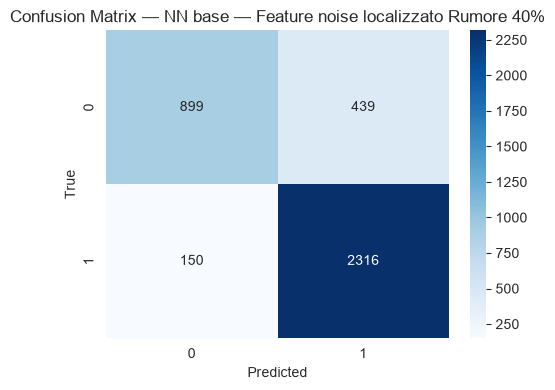
\includegraphics[height=3.9cm]{fnloc_nnbase_cm40}\hspace{0.8cm}
  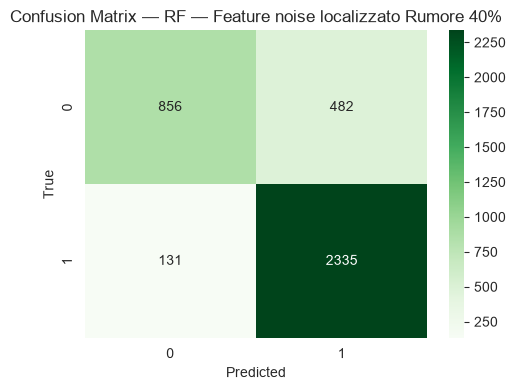
\includegraphics[height=3.9cm]{fnloc_rf_cm40}\\
  {\scriptsize Matrici di confusione al $40\%$: NN Base (sinistra) e Random Forest (destra).}
\end{frame}

\begin{frame}{Feature noise localizzato: curve di addestramento}
  \centering
  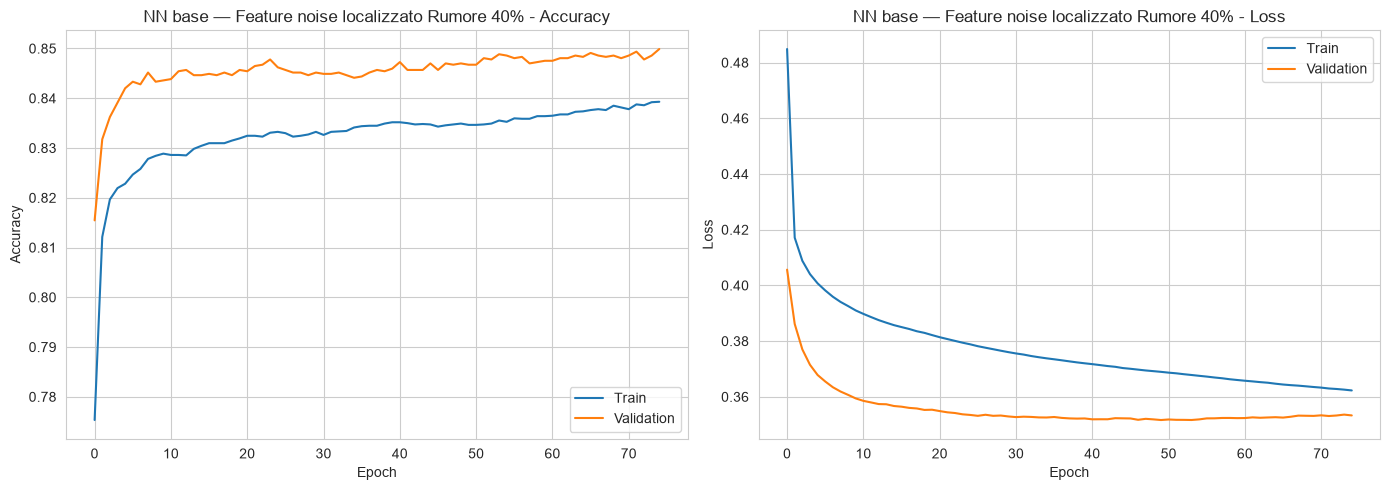
\includegraphics[height=3.3cm]{fnloc_nnbase_curve40}\hfill
  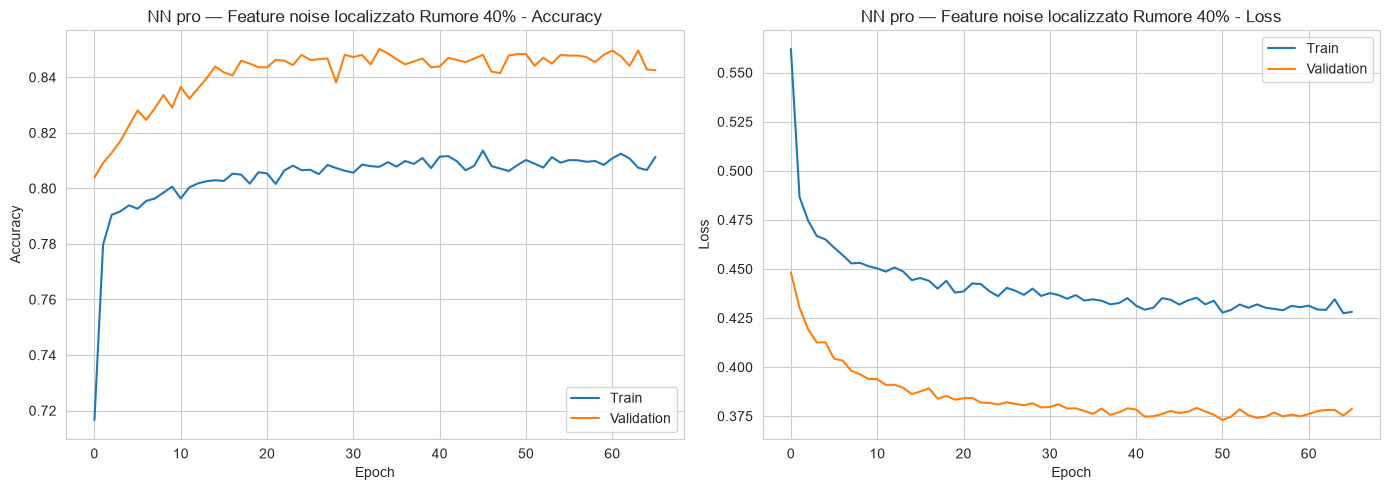
\includegraphics[height=3.3cm]{fnloc_nnpro_curve40}\\
  {\scriptsize Curve al $40\%$: NN Base (sinistra) vs NN Pro (destra).}
\end{frame}

\begin{frame}{Feature noise localizzato -- evidenze grafiche}
  \begin{columns}[c]
    \begin{column}{0.5\textwidth}
      \centering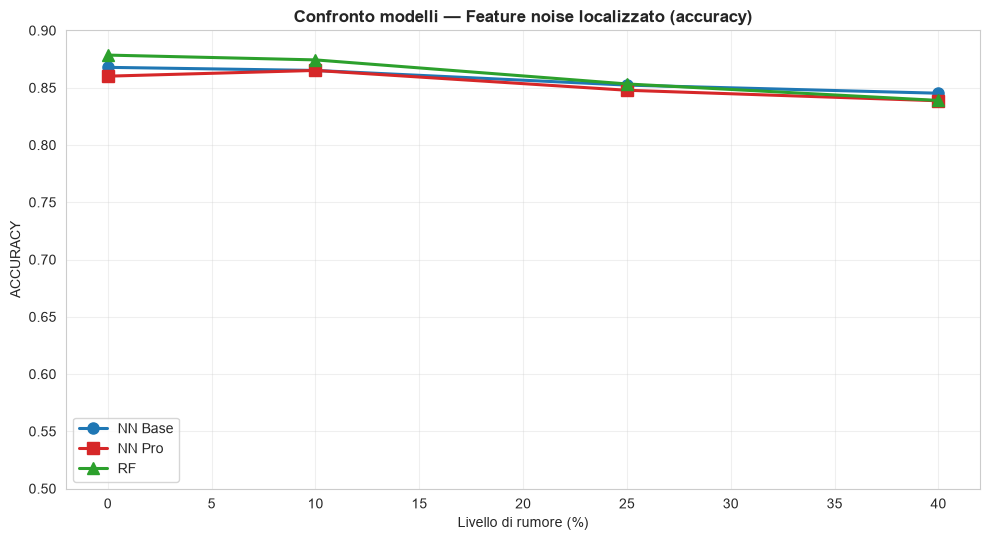
\includegraphics[height=3.0cm]{fnloc_compare_acc}\\
      {\scriptsize Accuratezza: curve vicine e quasi piatte.}
    \end{column}
    \begin{column}{0.5\textwidth}
      \centering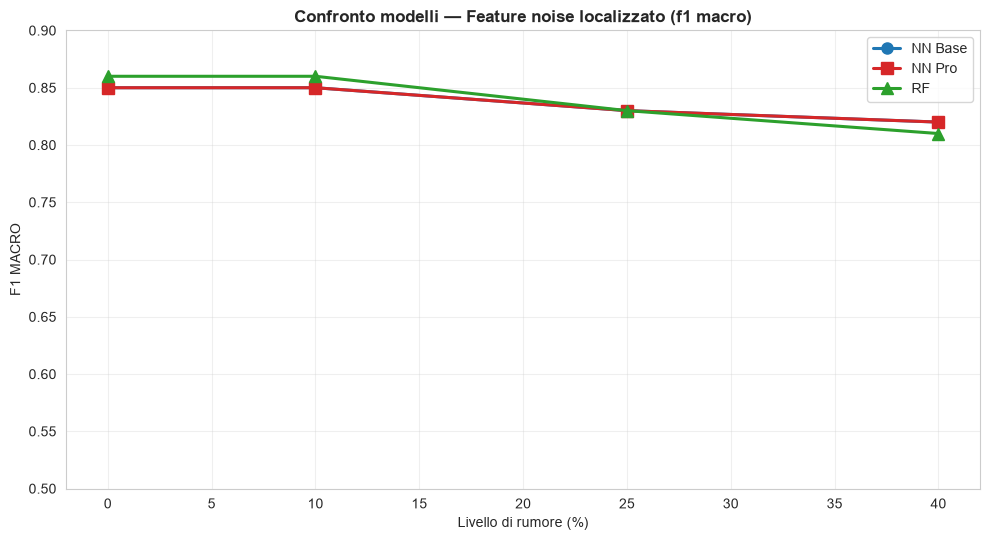
\includegraphics[height=3.0cm]{fnloc_compare_f1}\\
      {\scriptsize F1 macro: stesso andamento del rumore diffuso.}
    \end{column}
  \end{columns}
\end{frame}

% ---------- Label noise random ----------
\begin{frame}{Label noise random -- analisi}
  \begin{itemize}
    \item Fino al $25\%$ le metriche reggono; al $40\%$ il \textbf{crollo è
          netto}.
    \item Al $40\%$: NN Base $\to 0{,}7419$, RF $\to 0{,}7179$;
          la \textbf{NN Pro regge a $0{,}8044$}.
    \item Causa nelle learning curves: la Base \emph{memorizza} le etichette
          spurie (train $\approx 88\%$) mentre la validation pulita peggiora.
    \item L'\textbf{early stopping} della Pro ferma l'addestramento prima della
          memorizzazione del rumore $\Rightarrow$ validation $\approx 82\%$.
    \item Il RF memorizza le etichette errate nei nodi: errore distribuito su
          entrambe le classi.
  \end{itemize}
  \vfill
  \keypoint{Qui la regolarizzazione fa la differenza: monitorare i dati puliti
  protegge dal rumore sulle etichette.}
\end{frame}

\begin{frame}{Label noise random: metriche e matrici di confusione}
  \centering
  \footnotesize
  \begin{tabular}{c *{9}{c}}
    \toprule
     & \multicolumn{3}{c}{NN Base} & \multicolumn{3}{c}{NN Pro} & \multicolumn{3}{c}{Random Forest}\\
    \cmidrule(lr){2-4}\cmidrule(lr){5-7}\cmidrule(lr){8-10}
    Rumore & Acc & F1$_m$ & AUC & Acc & F1$_m$ & AUC & Acc & F1$_m$ & AUC \\
    \midrule
    Pulito & 0,8678 & 0,85 & 0,9214 & 0,8601 & 0,85 & 0,9238 & 0,8785 & 0,86 & 0,9300 \\
    10\% & 0,8623 & 0,84 & 0,9128 & 0,8570 & 0,84 & 0,9200 & 0,8767 & 0,86 & 0,9214 \\
    25\% & 0,8410 & 0,82 & 0,8882 & 0,8378 & 0,83 & 0,9081 & 0,8399 & 0,82 & 0,8884 \\
    40\% & 0,7419 & 0,69 & 0,7513 & \textbf{0,8044} & \textbf{0,79} & \textbf{0,8677} & 0,7179 & 0,70 & 0,7673 \\
    \bottomrule
  \end{tabular}
  \vspace{0.3cm}
  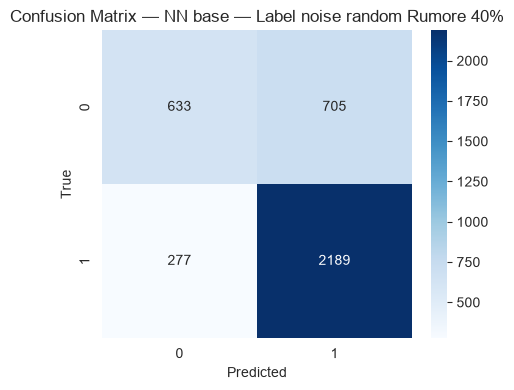
\includegraphics[height=3.9cm]{lnr_nnbase_cm40}\hfill
  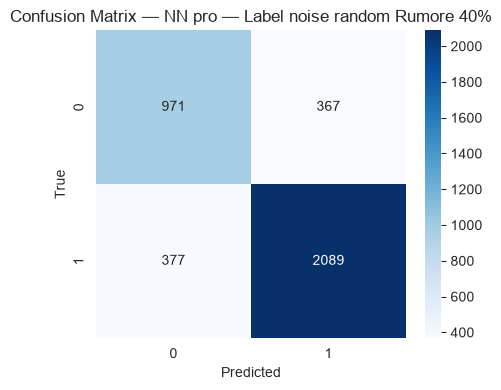
\includegraphics[height=3.9cm]{lnr_nnpro_cm40}\hfill
  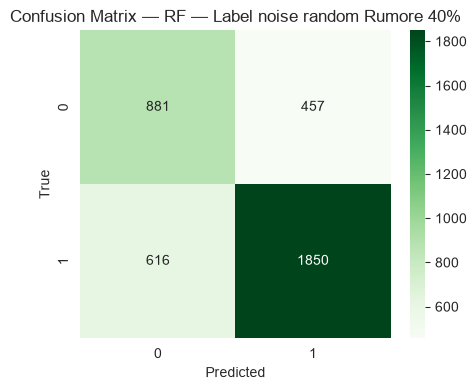
\includegraphics[height=3.9cm]{lnr_rf_cm40}\\
  {\scriptsize Matrici di confusione al $40\%$: NN Base, NN Pro, Random Forest.}
\end{frame}

\begin{frame}{Label noise random: curve di addestramento}
  \centering
  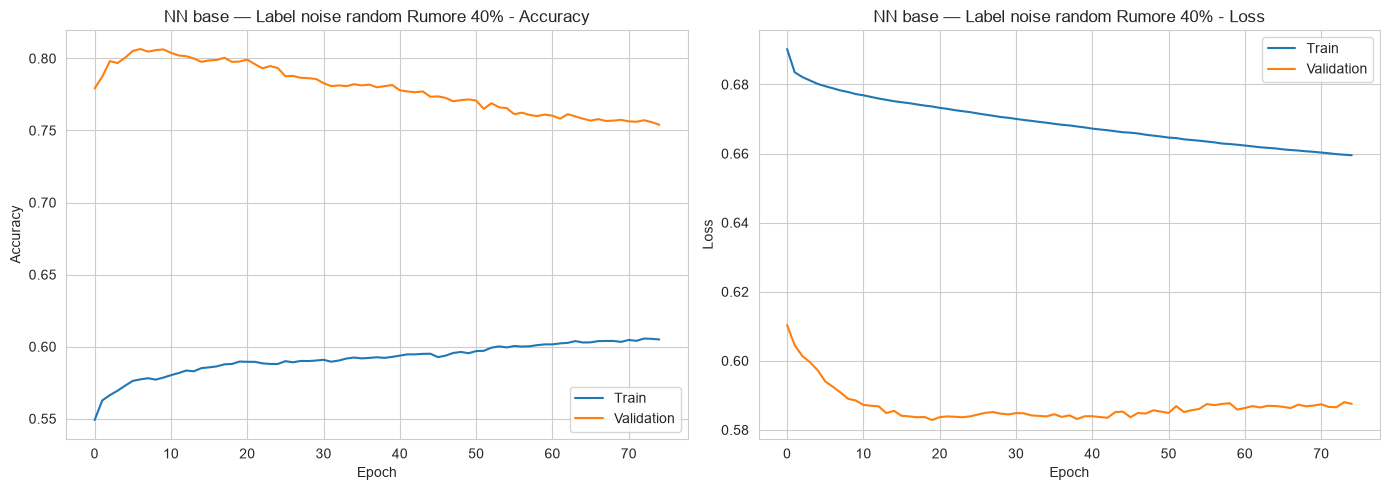
\includegraphics[height=3.3cm]{lnr_nnbase_curve40}\hfill
  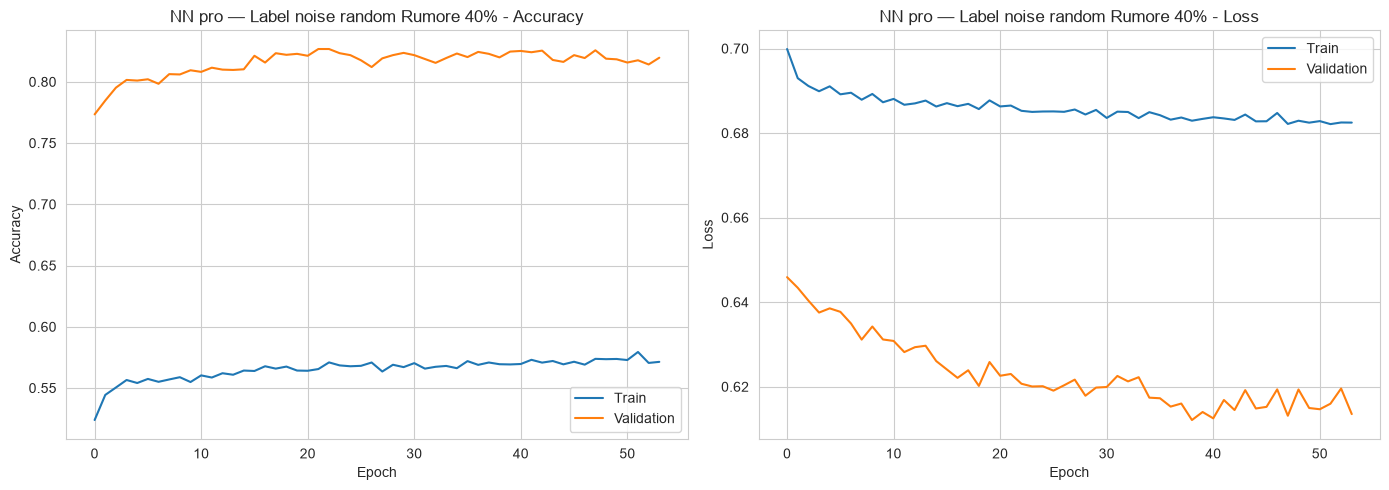
\includegraphics[height=3.3cm]{lnr_nnpro_curve40}\\
  {\scriptsize Curve al $40\%$: NN Base (sinistra) memorizza le etichette spurie
  (train sale, validation scende); NN Pro (destra) ferma l'addestramento con
  l'early stopping prima della memorizzazione.}
\end{frame}

\begin{frame}{Label noise random -- evidenze grafiche}
  \begin{columns}[c]
    \begin{column}{0.5\textwidth}
      \centering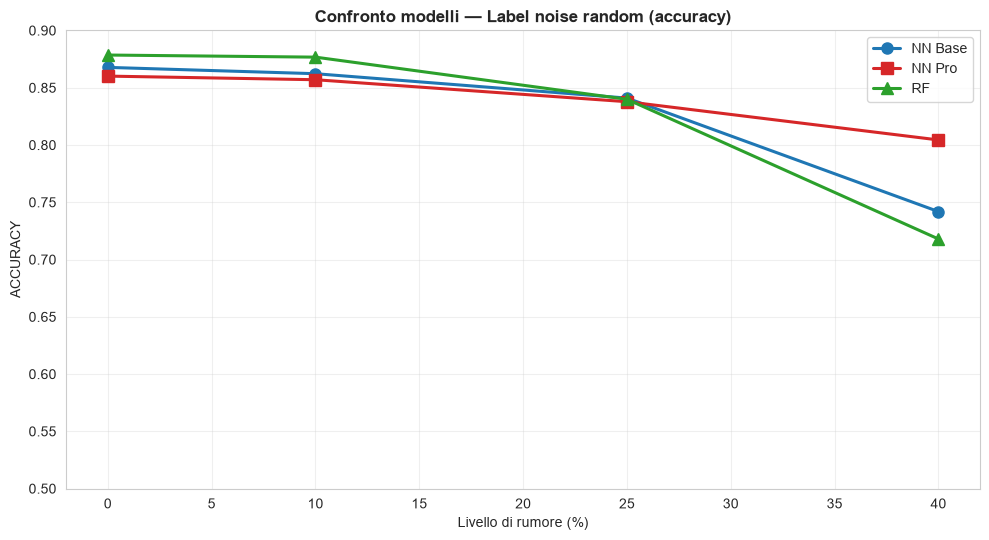
\includegraphics[height=4.0cm]{lnr_compare_acc}\\
    \end{column}
    \begin{column}{0.5\textwidth}
      \centering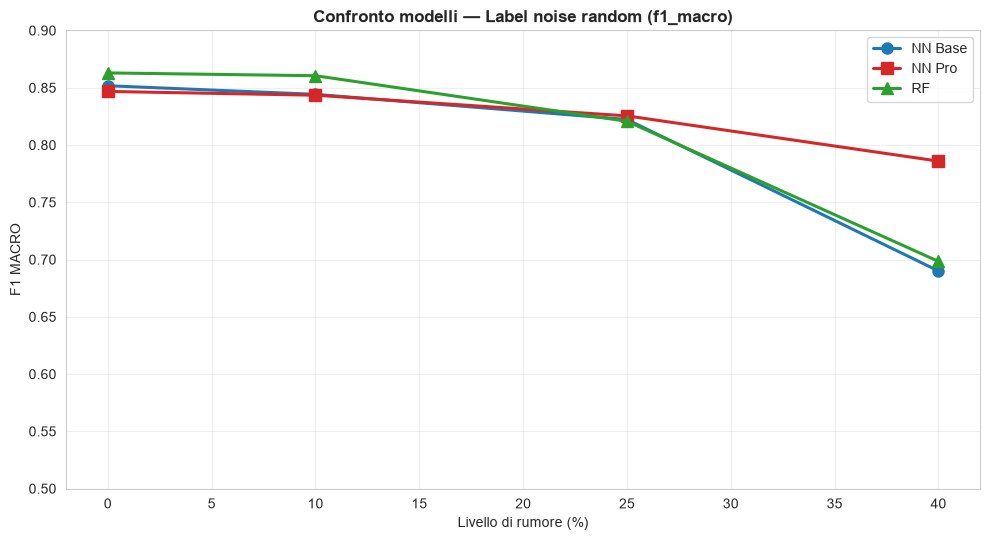
\includegraphics[height=4.0cm]{lnr_compare_f1}\\
    \end{column}
  \end{columns}
\end{frame}

% ---------- Label noise borderline ----------
\begin{frame}{Label noise borderline -- analisi}
  \begin{itemize}
    \item Il disturbo \textbf{più distruttivo}: cala già al $25\%$, al $40\%$
          tutti scendono attorno al \textbf{$60\%$}.
    \item Sotto la soglia del classificatore banale ($\sim 65\%$): i modelli
          diventano \textbf{attivamente fuorvianti}.
    \item Invertire i campioni vicini al confine \textbf{sposta il confine
          decisionale} appreso: è un errore sistematico, non varianza.
    \item Le learning curves della NN Pro non mostrano alcun vantaggio:
          regolarizzazione ed early stopping \textbf{non recuperano}.
    \item Danno \textbf{simmetrico} tra le classi: il ribilanciamento è vanificato.
    \item Log loss sul test al $40\%$: Base $1{,}06$, Pro $0{,}61$ $\Rightarrow$
          l'early stopping contiene almeno il danno sulla \textbf{calibrazione}.
  \end{itemize}
  \vfill
  \keypoint{A parità di flip, falsificare le istanze ambigue è molto più dannoso
  del rumore casuale: corrompe la struttura, non solo i dati.}
\end{frame}

\begin{frame}{Label noise borderline: metriche e matrici di confusione}
  \centering
  \footnotesize
  \begin{tabular}{c *{9}{c}}
    \toprule
     & \multicolumn{3}{c}{NN Base} & \multicolumn{3}{c}{NN Pro} & \multicolumn{3}{c}{Random Forest}\\
    \cmidrule(lr){2-4}\cmidrule(lr){5-7}\cmidrule(lr){8-10}
    Rumore & Acc & F1$_m$ & AUC & Acc & F1$_m$ & AUC & Acc & F1$_m$ & AUC \\
    \midrule
    Pulito & 0,8678 & 0,85 & 0,9214 & 0,8601 & 0,85 & 0,9238 & 0,8785 & 0,86 & 0,9300 \\
    10\% & 0,8252 & 0,80 & 0,8680 & 0,8352 & 0,82 & 0,8915 & 0,8383 & 0,81 & 0,8886 \\
    25\% & 0,7326 & 0,71 & 0,7879 & 0,7403 & 0,72 & 0,8265 & 0,7387 & 0,72 & 0,8043 \\
    40\% & 0,6002 & 0,59 & 0,6656 & \textbf{0,6354} & \textbf{0,62} & \textbf{0,7084} & 0,6094 & 0,60 & 0,6774 \\
    \bottomrule
  \end{tabular}
  \vspace{0.15cm}
  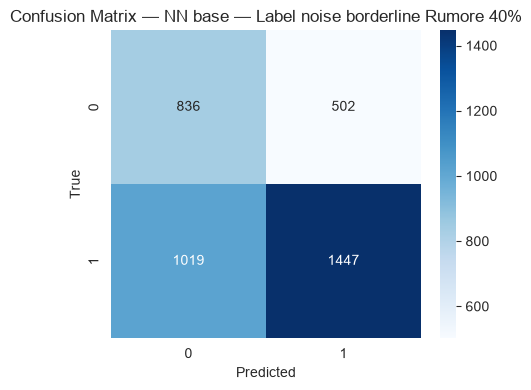
\includegraphics[height=3.5cm]{lnb_nnbase_cm40}\hfill
  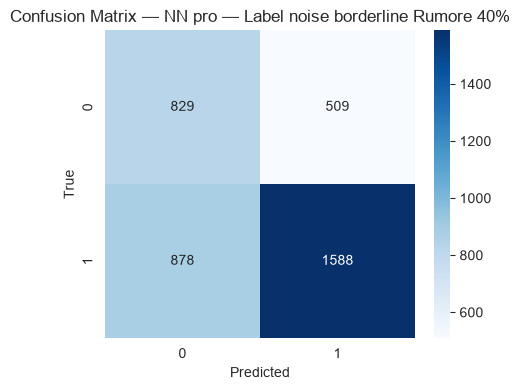
\includegraphics[height=3.5cm]{lnb_nnpro_cm40}\hfill
  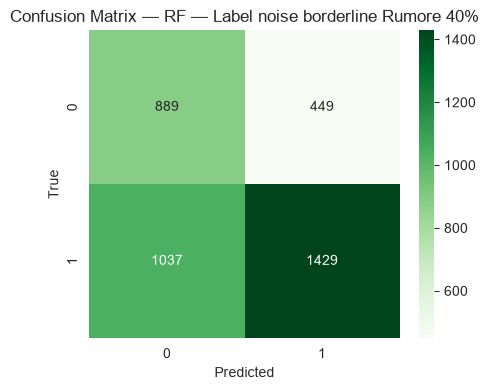
\includegraphics[height=3.5cm]{lnb_rf_cm40}\\
  {\scriptsize Matrici di confusione al $40\%$: NN Base, NN Pro, Random Forest -- errori diffusi in modo simmetrico.}
\end{frame}

\begin{frame}{Label noise borderline: curve di addestramento}
  \centering
  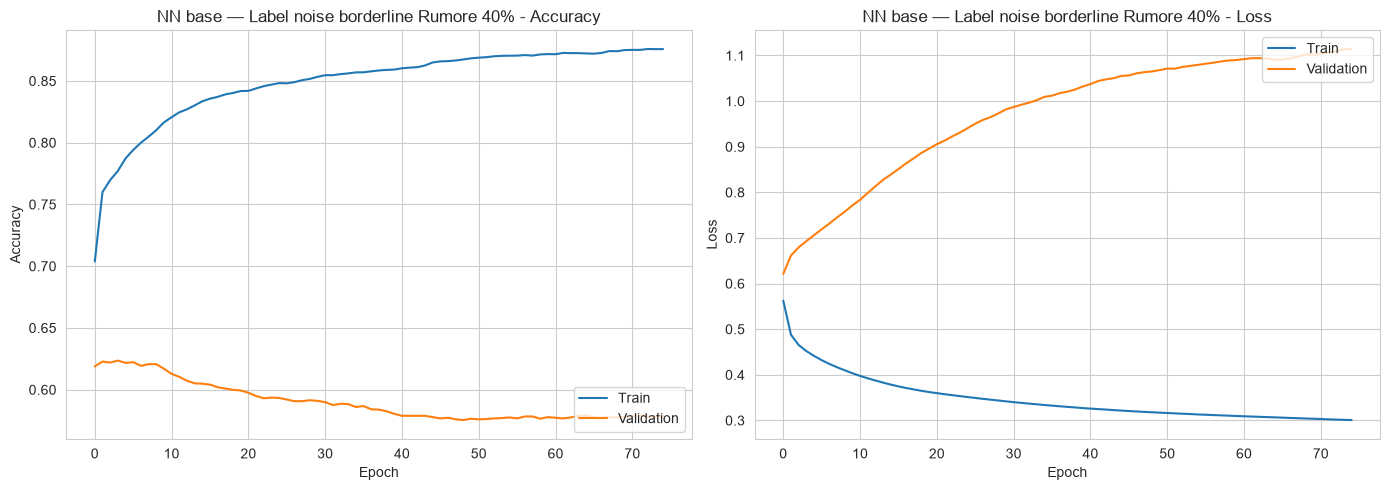
\includegraphics[height=3.3cm]{lnb_nnbase_curve40}\hfill
  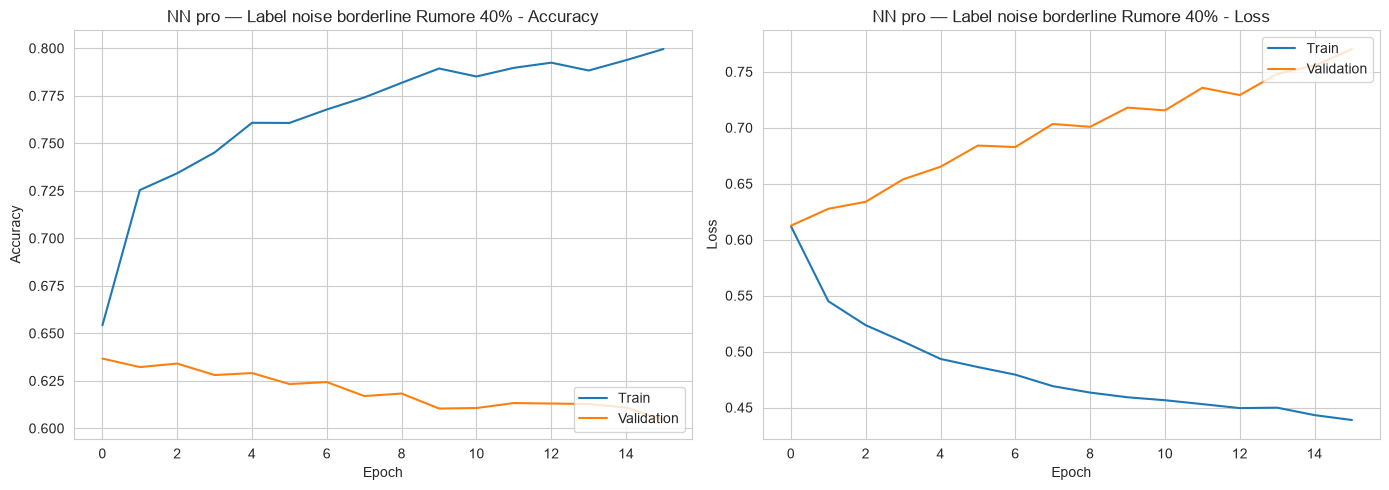
\includegraphics[height=3.3cm]{lnb_nnpro_curve40}\\
  {\scriptsize Curve al $40\%$: NN Base (sinistra) e NN Pro (destra) -- crolla anche
  la validation, l'early stopping non offre alcun vantaggio.}
\end{frame}

\begin{frame}{Label noise borderline -- evidenze grafiche}
  \begin{columns}[c]
    \begin{column}{0.5\textwidth}
      \centering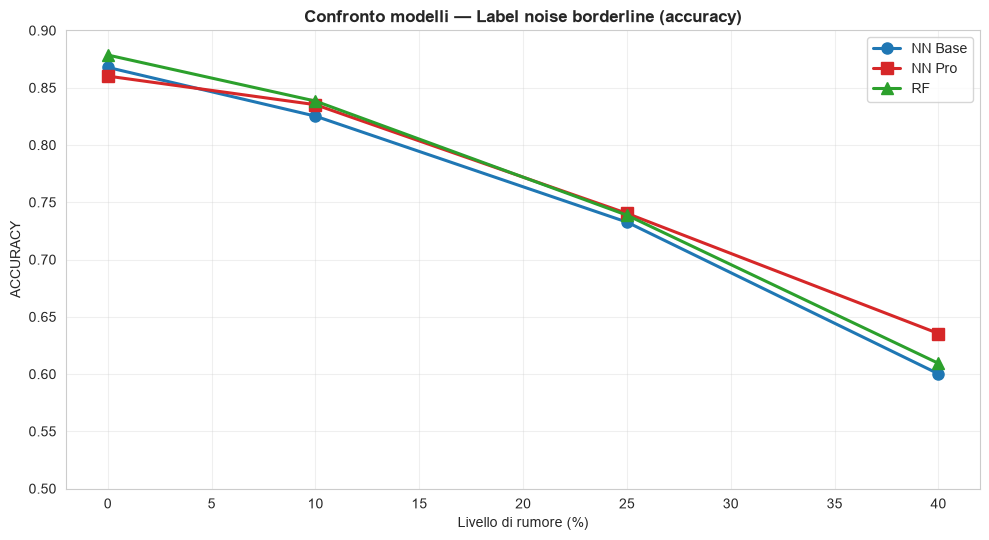
\includegraphics[height=4.0cm]{lnb_compare_acc}\\
      {\scriptsize Al $40\%$ tutti convergono verso il $60\%$: collasso predittivo.}
    \end{column}
    \begin{column}{0.5\textwidth}
      \centering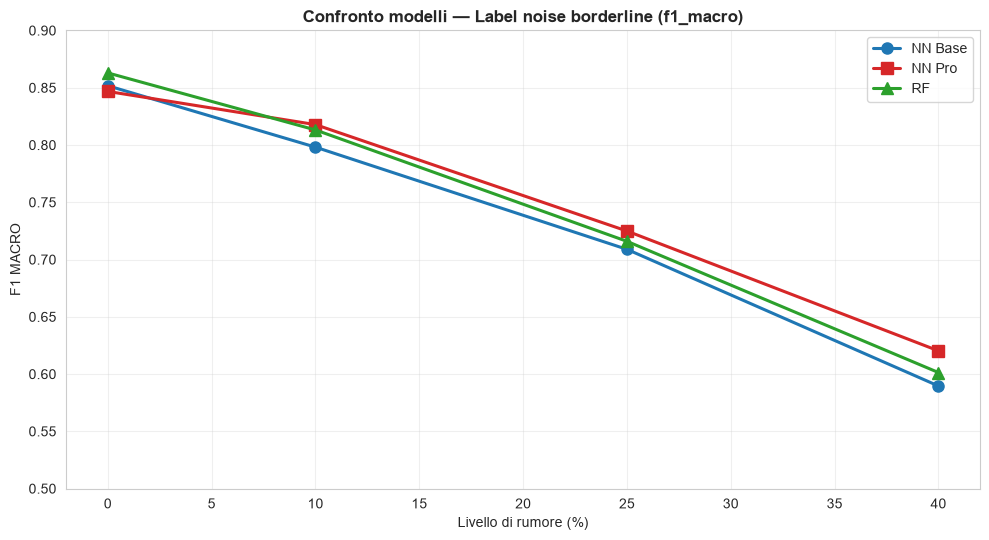
\includegraphics[height=4.0cm]{lnb_compare_f1}\\
    \end{column}
  \end{columns}
\end{frame}

% ---------- Missing values ----------
\begin{frame}{Missing values -- analisi}
  \begin{itemize}
    \item Celle sostituite con \texttt{NaN}; i modelli non leggono dati incompleti
          $\Rightarrow$ serve \textbf{imputazione}.
    \item Con la mediana (variante canonica) le metriche restano $82$--$85\%$:
          degrado \textbf{lineare e gestibile}.
    \item Il \textbf{Random Forest} è il più resistente ($0{,}8528$ al $40\%$):
          opera per divisioni, isola meglio le celle imputate.
    \item \textbf{Media vs mediana}: divario marginale e senza direzione univoca.
          \begin{itemize}
            \item[$\circ$] mediana lievemente meglio sulla Base ad alta corruzione;
            \item[$\circ$] media leggermente meglio sulla Pro; pari sul RF.
          \end{itemize}
  \end{itemize}
  \vfill
  \keypoint{La mediana resta riferimento per robustezza teorica alle code, ma sul
  piano empirico la scelta incide poco.}
\end{frame}

\begin{frame}{Missing values: metriche e matrici di confusione}
  \centering
  \footnotesize
  \begin{tabular}{c *{9}{c}}
    \toprule
     & \multicolumn{3}{c}{NN Base} & \multicolumn{3}{c}{NN Pro} & \multicolumn{3}{c}{Random Forest}\\
    \cmidrule(lr){2-4}\cmidrule(lr){5-7}\cmidrule(lr){8-10}
    Rumore & Acc & F1$_m$ & AUC & Acc & F1$_m$ & AUC & Acc & F1$_m$ & AUC \\
    \midrule
    Pulito & 0,8678 & 0,85 & 0,9214 & 0,8601 & 0,85 & 0,9238 & 0,8785 & 0,86 & 0,9300 \\
    10\% & 0,8617 & 0,84 & 0,9172 & 0,8570 & 0,84 & 0,9190 & 0,8720 & 0,85 & 0,9208 \\
    25\% & 0,8425 & 0,83 & 0,9057 & 0,8328 & 0,82 & 0,9046 & 0,8578 & 0,84 & 0,9129 \\
    40\% & 0,8328 & 0,81 & 0,8915 & 0,8226 & 0,81 & 0,8937 & \textbf{0,8528} & \textbf{0,83} & \textbf{0,9039} \\
    \bottomrule
  \end{tabular}
  \vspace{0.15cm}
  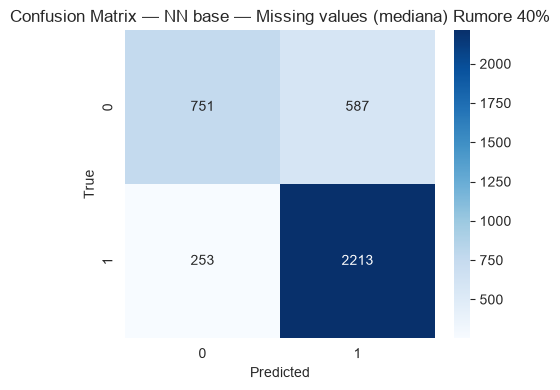
\includegraphics[height=3.9cm]{mv_nnbase_cm40}\hspace{0.8cm}
  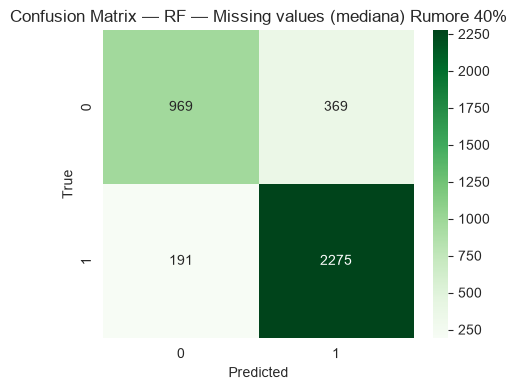
\includegraphics[height=3.9cm]{mv_rf_cm40}\\
  {\scriptsize Matrici al $40\%$: NN Base (sinistra) e RF (destra); gli errori pesano sugli adroni.}
\end{frame}

\begin{frame}{Missing values: curve di addestramento}
  \centering
  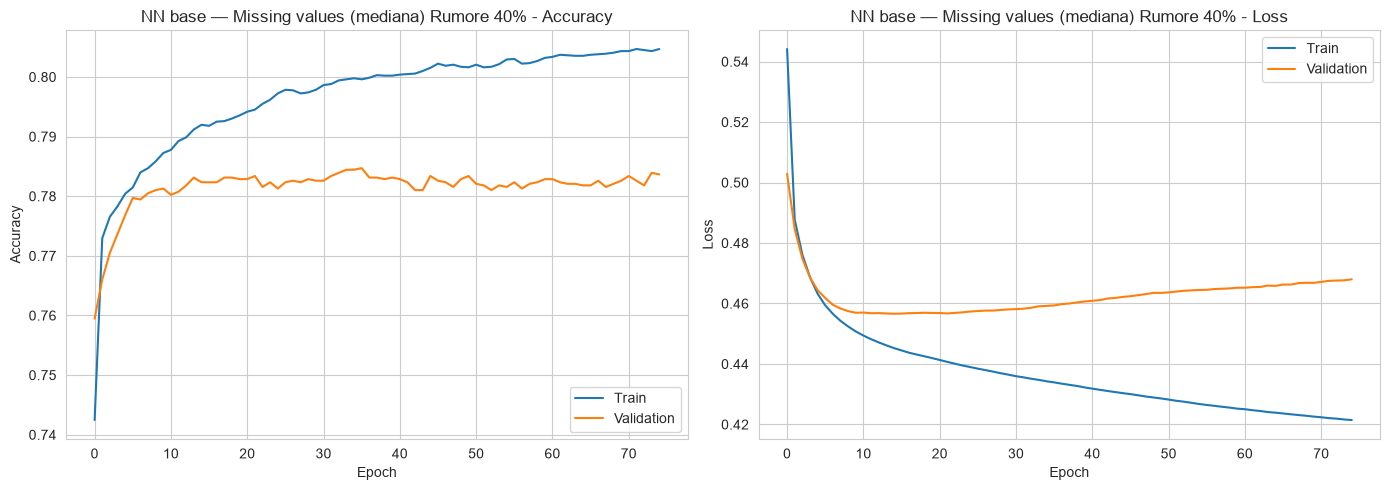
\includegraphics[height=4.5cm]{mv_nnbase_curve40}\\
  {\scriptsize NN Base al $40\%$ di valori mancanti: convergenza regolare, nessun
  overfitting marcato.}
\end{frame}

\begin{frame}{Missing values -- evidenze grafiche}
  \begin{columns}[c]
    \begin{column}{0.5\textwidth}
      \centering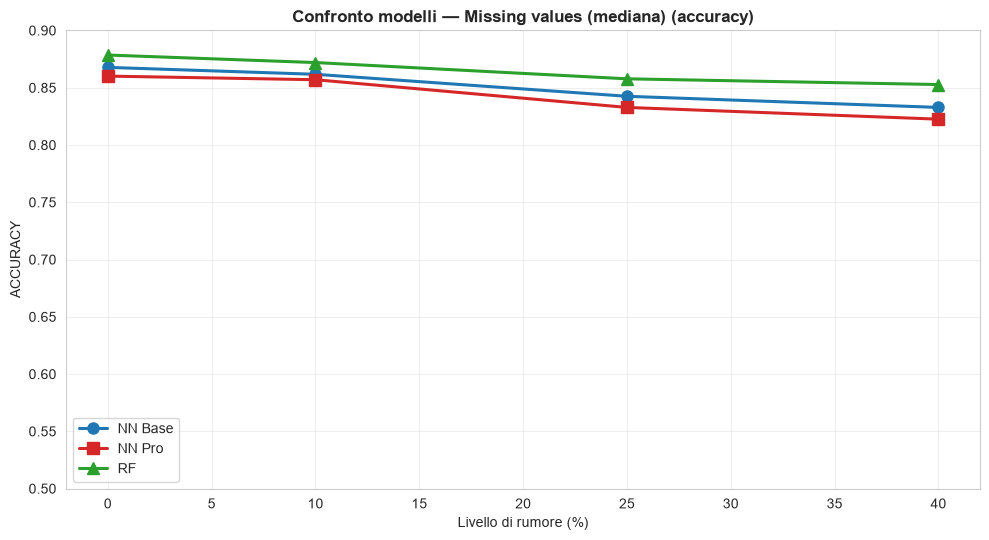
\includegraphics[height=4.0cm]{mv_compare_acc}\\
      {\scriptsize Imputazione mediana: RF in vantaggio costante.}
    \end{column}
    \begin{column}{0.5\textwidth}
      \centering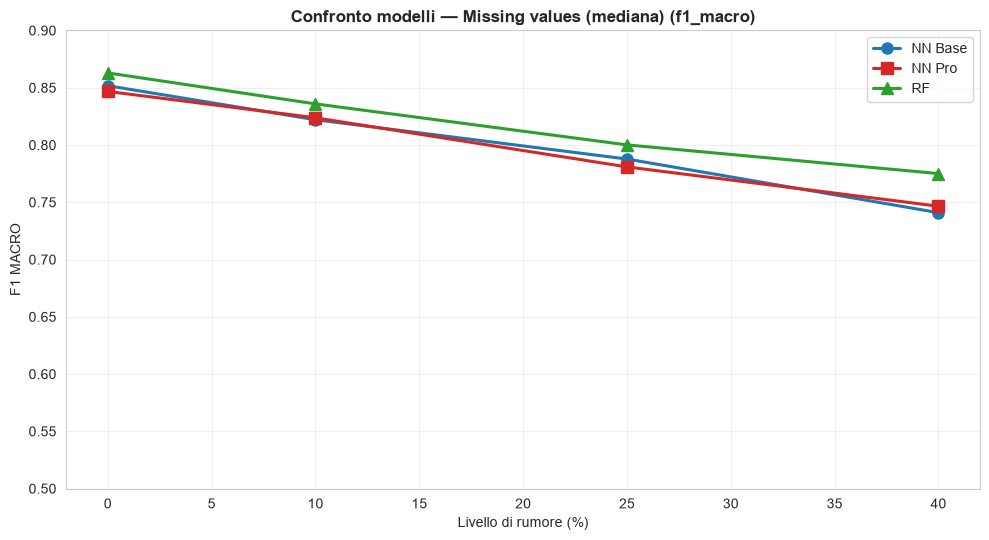
\includegraphics[height=4.0cm]{mv_compare_f1}\\
    \end{column}
  \end{columns}
\end{frame}

% ---------- Outlier ----------
\begin{frame}{Outlier -- analisi}
  \begin{itemize}
    \item Il disturbo \textbf{meno dannoso}: l'accuratezza resta $85$--$87\%$,
          quasi nessuna tendenza al degrado.
    \item Motivo \textbf{nella natura del disturbo}, non nel trattamento: i valori
          $\pm 5\sigma$ hanno segno casuale e scorrelato dall'etichetta
          $\Rightarrow$ il loro contributo al gradiente si media a zero.
    \item Tre strategie quasi equivalenti: nessun trattamento, winsorizzazione,
          imputazione.
    \item Ad alta corruzione la winsorizzazione al $5\%$ è in gran parte
          \textbf{inefficace} (i percentili stessi sono saturati).
  \end{itemize}
  \vfill
  \keypoint{La robustezza nasce dalla \textbf{natura poco dannosa del disturbo}
  più che dalla mitigazione; teniamo la winsorizzazione per prudenza.}
\end{frame}

\begin{frame}{Outlier: metriche e matrici di confusione}
  \centering
  \footnotesize
  \begin{tabular}{c *{9}{c}}
    \toprule
     & \multicolumn{3}{c}{NN Base} & \multicolumn{3}{c}{NN Pro} & \multicolumn{3}{c}{Random Forest}\\
    \cmidrule(lr){2-4}\cmidrule(lr){5-7}\cmidrule(lr){8-10}
    Rumore & Acc & F1$_m$ & AUC & Acc & F1$_m$ & AUC & Acc & F1$_m$ & AUC \\
    \midrule
    Pulito & 0,8678 & 0,85 & 0,9214 & 0,8601 & 0,85 & 0,9238 & 0,8785 & 0,86 & 0,9300 \\
    10\% & 0,8657 & 0,85 & 0,9196 & 0,8583 & 0,84 & 0,9220 & \textbf{0,8788} & \textbf{0,86} & \textbf{0,9295} \\
    25\% & 0,8628 & 0,84 & 0,9160 & 0,8441 & 0,83 & 0,9173 & 0,8751 & 0,86 & 0,9267 \\
    40\% & 0,8615 & 0,84 & 0,9116 & 0,8541 & 0,84 & 0,9201 & 0,8736 & 0,86 & 0,9250 \\
    \bottomrule
  \end{tabular}
  \vspace{0.15cm}
  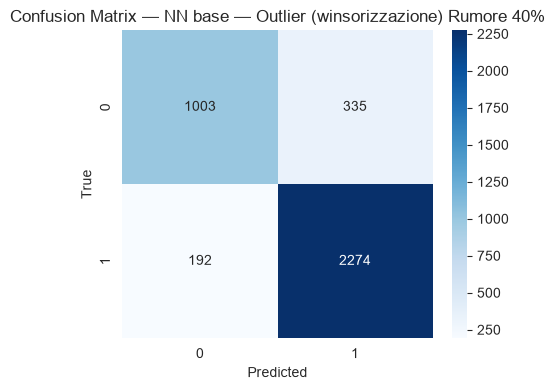
\includegraphics[height=3.9cm]{out_nnbase_cm40}\hspace{0.8cm}
  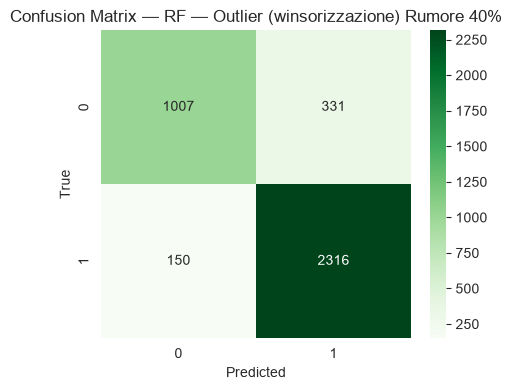
\includegraphics[height=3.9cm]{out_rf_cm40}\\
  {\scriptsize Matrici al $40\%$: prestazioni indistinguibili dal caso pulito.}
\end{frame}

\begin{frame}{Outlier: curve di addestramento}
  \centering
  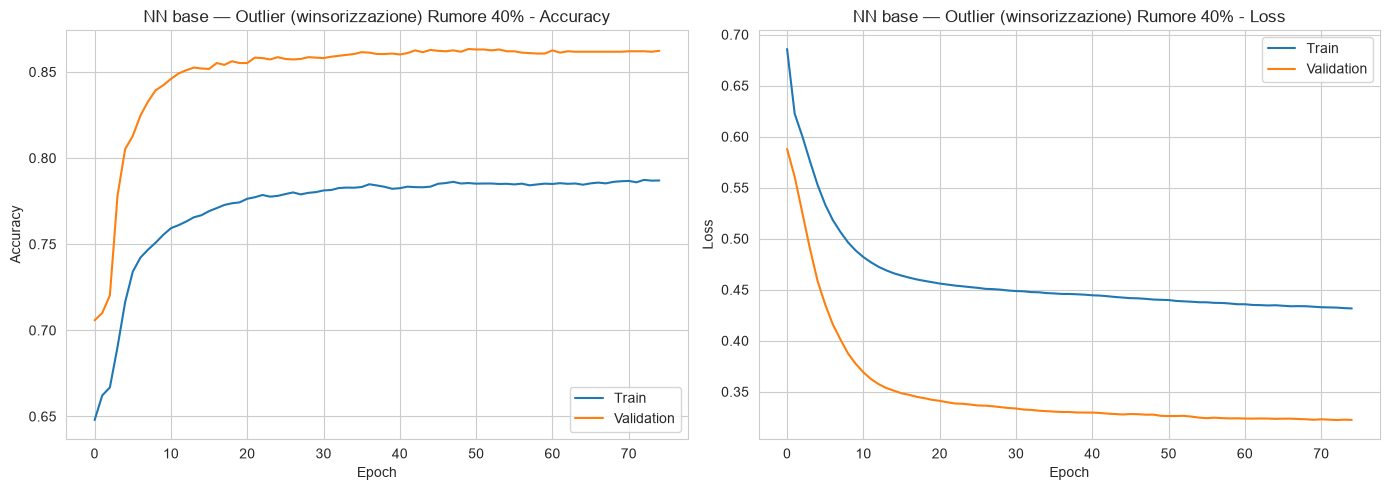
\includegraphics[height=4.5cm]{out_nnbase_curve40}\\
  {\scriptsize NN Base al $40\%$ di outlier: convergenza regolare, nessun impatto
  visibile sull'addestramento.}
\end{frame}

\begin{frame}{Outlier -- evidenze grafiche}
  \begin{columns}[c]
    \begin{column}{0.5\textwidth}
      \centering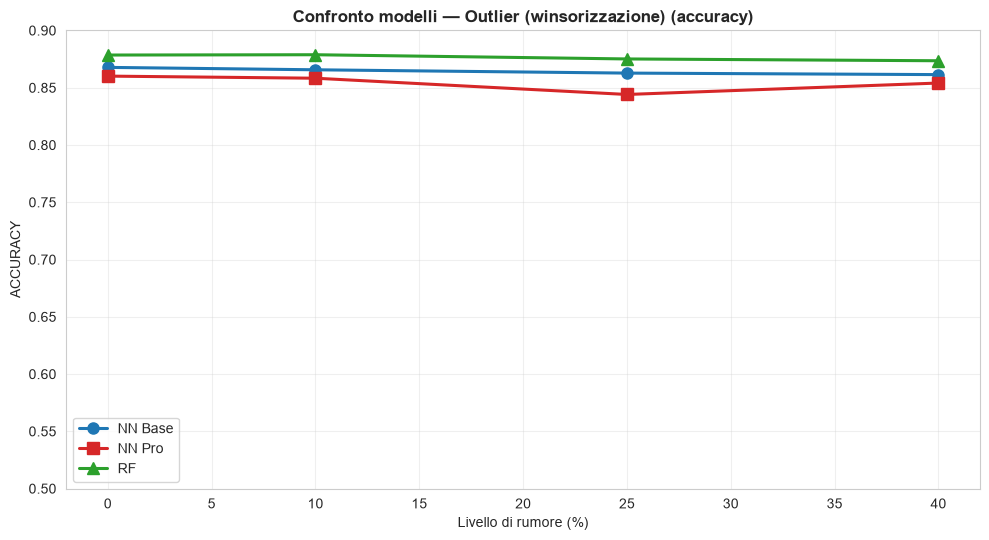
\includegraphics[height=4.0cm]{out_compare_acc}\\
      {\scriptsize Winsorizzazione: curve pressoché piatte.}
    \end{column}
    \begin{column}{0.5\textwidth}
      \centering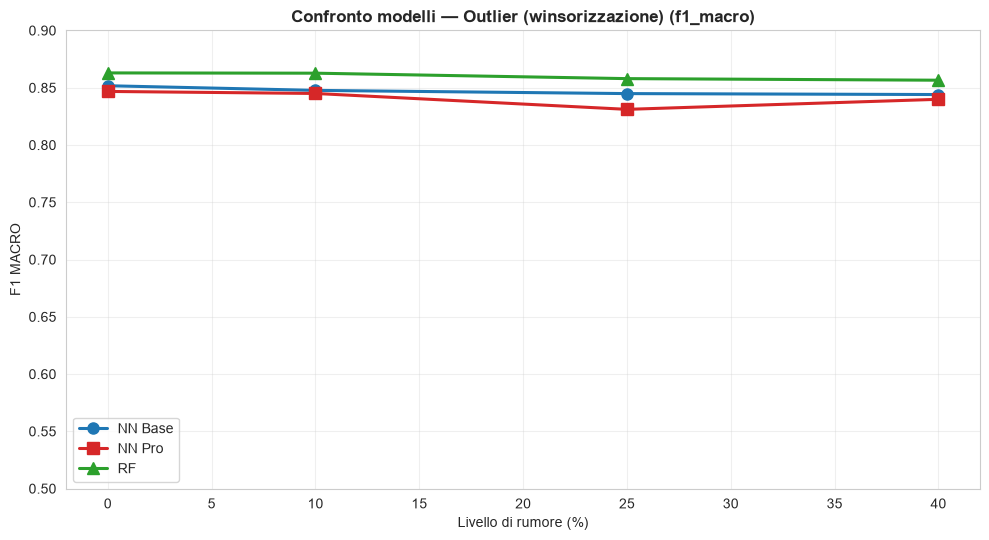
\includegraphics[height=4.0cm]{out_compare_f1}\\
    \end{column}
  \end{columns}
\end{frame}

% ---------- Missing feature ----------
\begin{frame}{Missing feature (sensore guasto) -- analisi}
  \begin{itemize}
    \item Intere colonne azzerate su \emph{tutti} i set, per importanza:
          top-1 (\feat{fAlpha}) $\to$ top-3 $\to$ top-5.
    \item Esito \textbf{molto grave}: già al $10\%$ un calo di $4$--$5$ punti; al
          $40\%$ tutti attorno al $70\%$.
    \item Qui non c'è rumore da filtrare ma \textbf{informazione che non esiste
          più}: azzerare \feat{fAlpha} pesa più del feature noise massimo.
    \item \textbf{Controtendenza}: la NN Pro è la \emph{meno} robusta
          ($0{,}6995$ al $40\%$): le difese contro l'overfitting irrigidiscono il
          modello quando manca informazione.
  \end{itemize}
  \vfill
  \keypoint{\feat{fAlpha} è scorrelata dalle altre: la sua perdita è
  \textbf{insostituibile} e colpisce soprattutto gli adroni.}
\end{frame}

\begin{frame}{Missing feature: metriche e matrici di confusione}
  \centering
  \footnotesize
  \begin{tabular}{c *{9}{c}}
    \toprule
     & \multicolumn{3}{c}{NN Base} & \multicolumn{3}{c}{NN Pro} & \multicolumn{3}{c}{Random Forest}\\
    \cmidrule(lr){2-4}\cmidrule(lr){5-7}\cmidrule(lr){8-10}
    Rumore & Acc & F1$_m$ & AUC & Acc & F1$_m$ & AUC & Acc & F1$_m$ & AUC \\
    \midrule
    Pulito & 0,8678 & 0,85 & 0,9214 & 0,8601 & 0,85 & 0,9238 & 0,8785 & 0,86 & 0,9300 \\
    10\% & 0,8215 & 0,79 & 0,8675 & 0,8052 & 0,79 & 0,8716 & \textbf{0,8294} & \textbf{0,80} & \textbf{0,8788} \\
    25\% & 0,7773 & 0,74 & 0,8007 & 0,7574 & 0,73 & 0,7991 & 0,7836 & 0,75 & 0,8195 \\
    40\% & 0,7303 & 0,67 & 0,7413 & 0,6995 & 0,67 & 0,7347 & 0,7363 & 0,68 & 0,7494 \\
    \bottomrule
  \end{tabular}
  \vspace{0.15cm}
  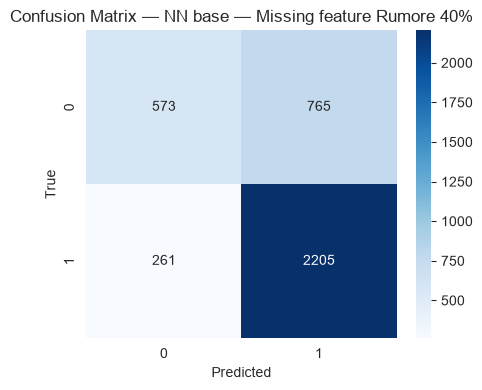
\includegraphics[height=3.5cm]{mf_nnbase_cm40}\hfill
  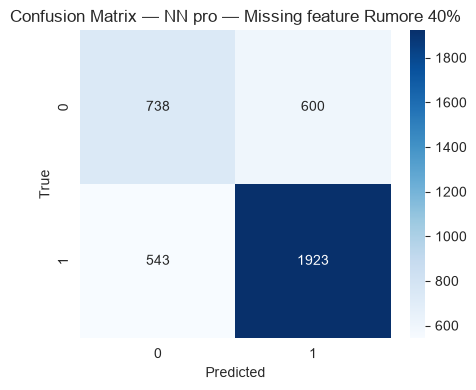
\includegraphics[height=3.5cm]{mf_nnpro_cm40}\hfill
  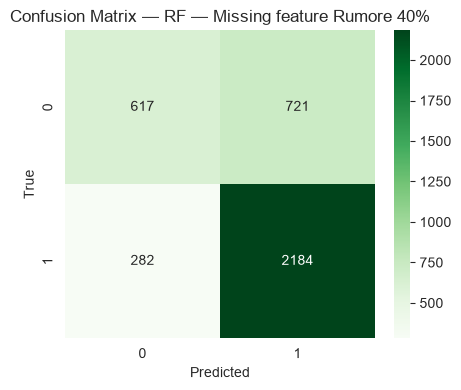
\includegraphics[height=3.5cm]{mf_rf_cm40}\\
  {\scriptsize Matrici di confusione al $40\%$ (top-5 feature rimosse): NN Base, NN Pro,
  Random Forest -- discriminazione adroni quasi azzerata.}
\end{frame}

\begin{frame}{Missing feature: curve di addestramento}
  \centering
  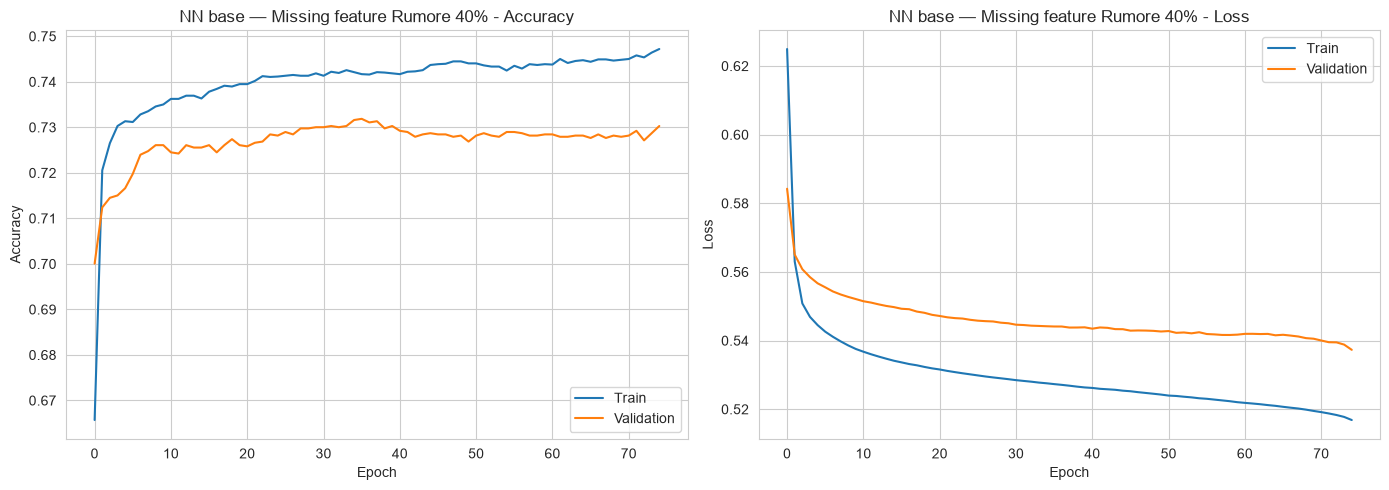
\includegraphics[height=3.3cm]{mf_nnbase_curve40}\hfill
  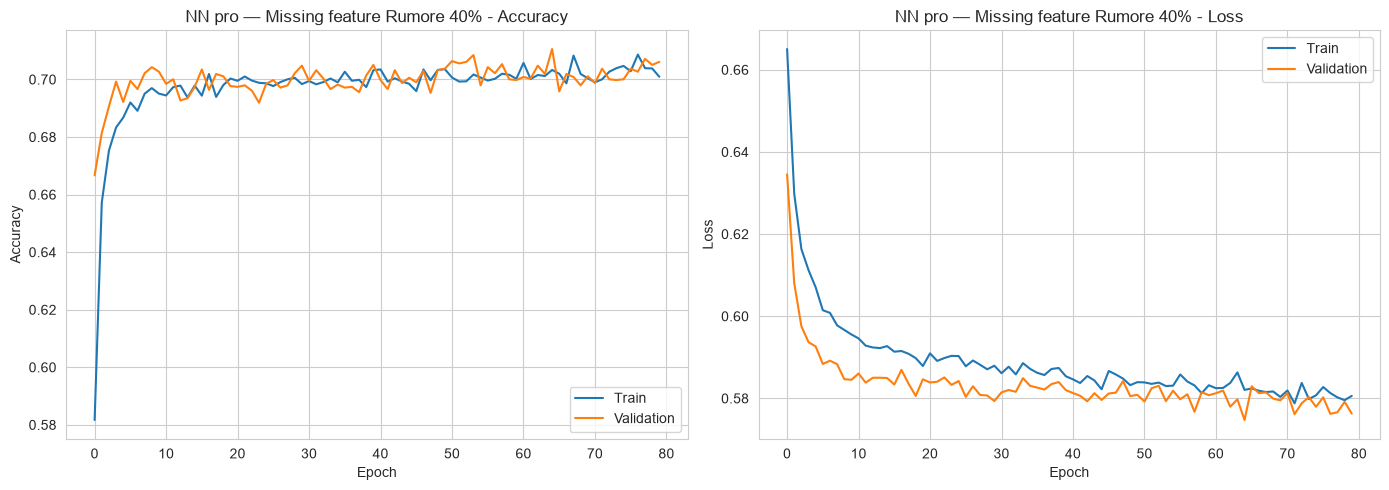
\includegraphics[height=3.3cm]{mf_nnpro_curve40}\\
  {\scriptsize Curve al $40\%$ (top-5 feature rimosse): NN Base (sinistra) e NN Pro
  (destra) -- la Pro, più rigida, non compensa l'informazione mancante.}
\end{frame}

\begin{frame}{Missing feature -- evidenze grafiche}
  \begin{columns}[c]
    \begin{column}{0.5\textwidth}
      \centering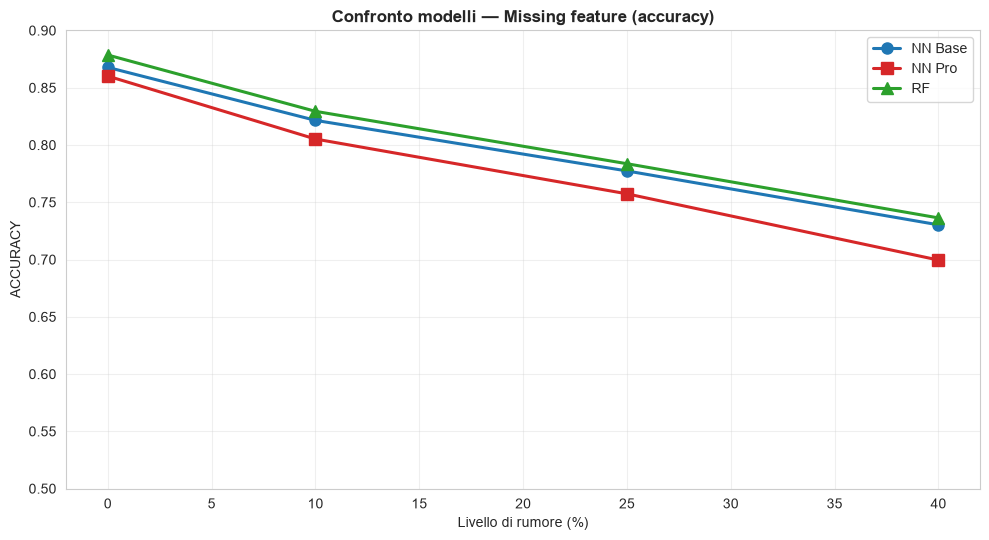
\includegraphics[height=4.0cm]{mf_compare_acc}\\
      {\scriptsize Rimuovere \feat{fAlpha}: declino severo dal primo step.}
    \end{column}
    \begin{column}{0.5\textwidth}
      \centering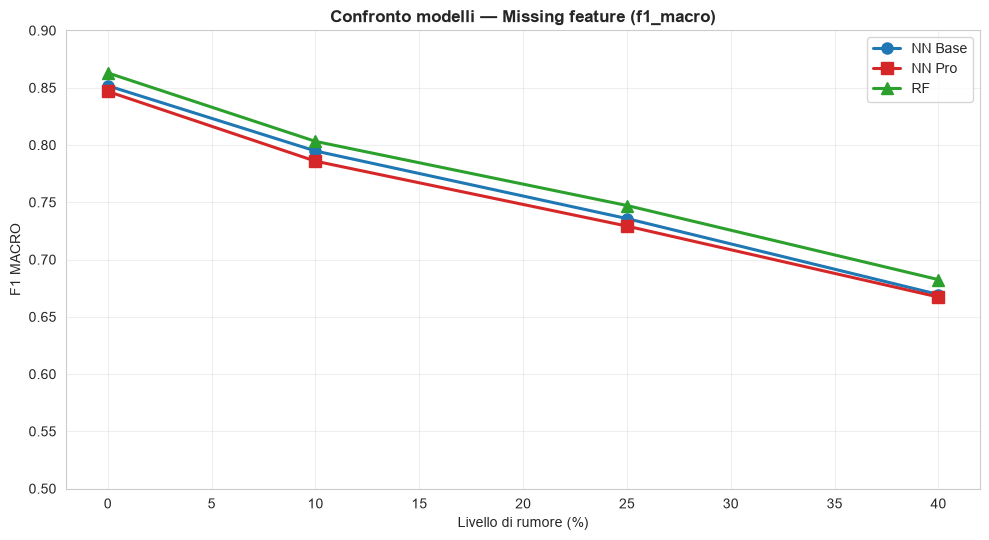
\includegraphics[height=4.0cm]{mf_compare_f1}\\
    \end{column}
  \end{columns}
\end{frame}

% ============================================================
\section{Controllo multi-seed}
% ============================================================
\begin{frame}{Controllo multi-seed: il trend è reale?}
  \begin{columns}[c]
    \begin{column}{0.5\textwidth}
      \centering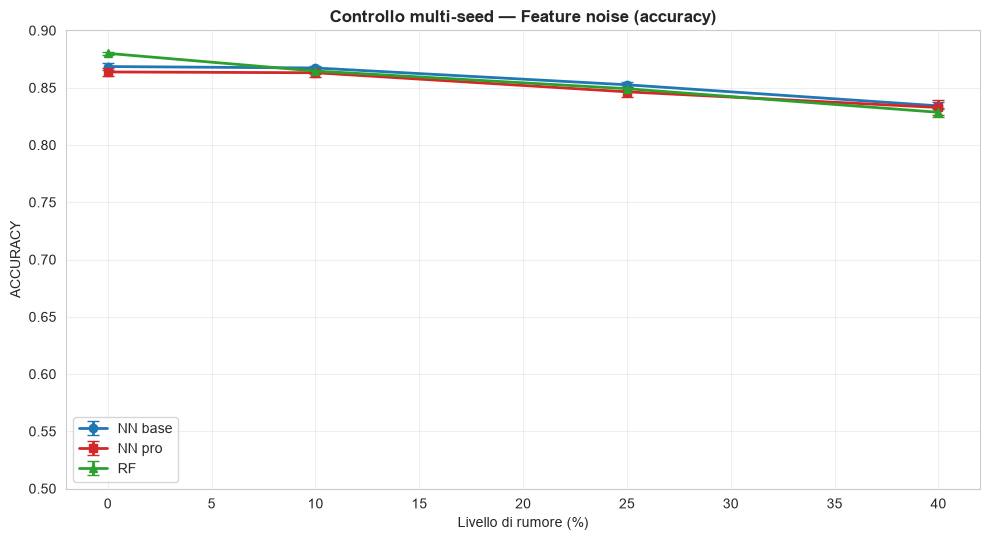
\includegraphics[width=\linewidth]{ms_acc}
    \end{column}
    \begin{column}{0.5\textwidth}
      \begin{itemize}
        \item Feature noise ripetuto su \textbf{cinque semi}
              $\{42, 7, 123, 2024, 99\}$.
        \item Ogni seme governa rumore, split e inizializzazione.
        \item Deviazione standard sempre $< 0{,}007$ (max $0{,}0068$).
        \item Un ordine di grandezza \textbf{sotto} il calo dovuto al rumore
              ($\sim 3{,}4$ punti per la NN Base).
      \end{itemize}
    \end{column}
  \end{columns}
  \vfill
  \keypoint{Le barre d'errore sono quasi impercettibili: il degrado è un
  \textbf{segnale reale}, non varianza procedurale.}
\end{frame}

\begin{frame}{Multi-seed -- F1 macro e gerarchia confermata}
  \begin{columns}[c]
    \begin{column}{0.55\textwidth}
      \centering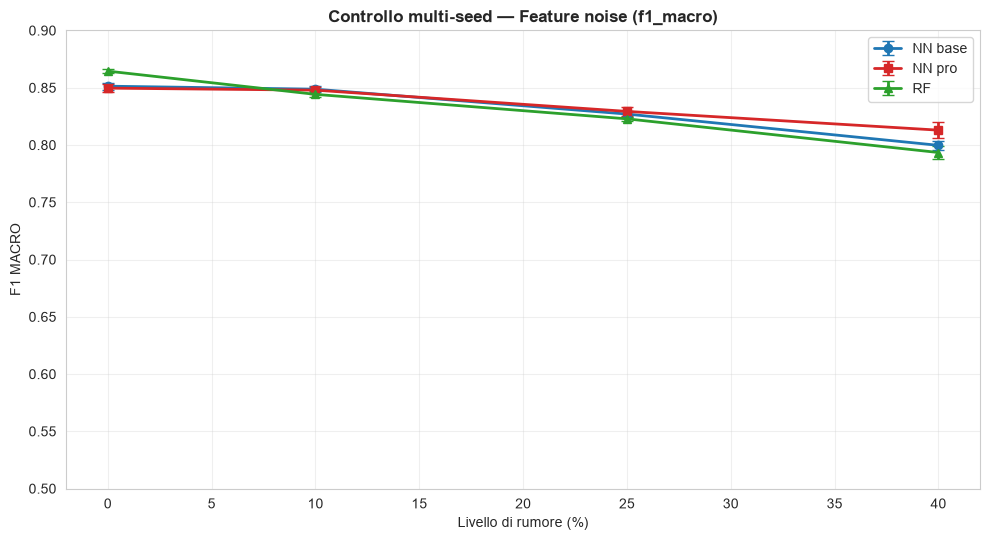
\includegraphics[width=\linewidth]{ms_f1}
    \end{column}
    \begin{column}{0.45\textwidth}
      \begin{itemize}
        \item Stesso ordinamento sulla metrica bilanciata.
        \item RF parte più in alto ($0{,}8800$) ma cede più rapidamente.
        \item La NN Pro ha il degrado \textbf{più graduale}.
        \item Le differenze sono coerenti tra i cinque semi.
      \end{itemize}
    \end{column}
  \end{columns}
  \vfill
  \keypoint{L'ordinamento osservato non dipende dalle fluttuazioni del generatore
  stocastico.}
\end{frame}

% ============================================================
\section{Sintesi e confronto tra modelli}
% ============================================================
\begin{frame}{Gerarchia di pericolosità dei rumori}
  \centering
  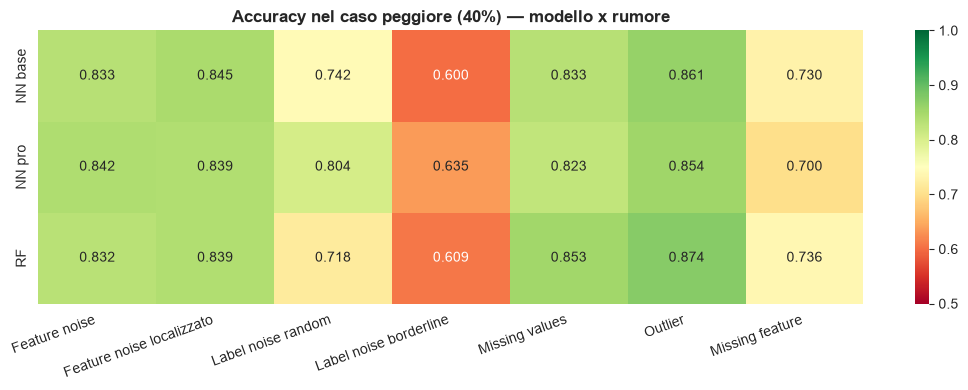
\includegraphics[width=0.92\textwidth]{summary_heatmap}\\
  \vspace{0.2cm}
  {\small outlier $<$ feature noise $\approx$ missing values $<$ label noise random
  $\approx$ missing feature $<$ \textbf{label noise borderline}.}
\end{frame}

\begin{frame}{Degradazione e ranking complessivo}
  \begin{columns}[c]
    \begin{column}{0.58\textwidth}
      \centering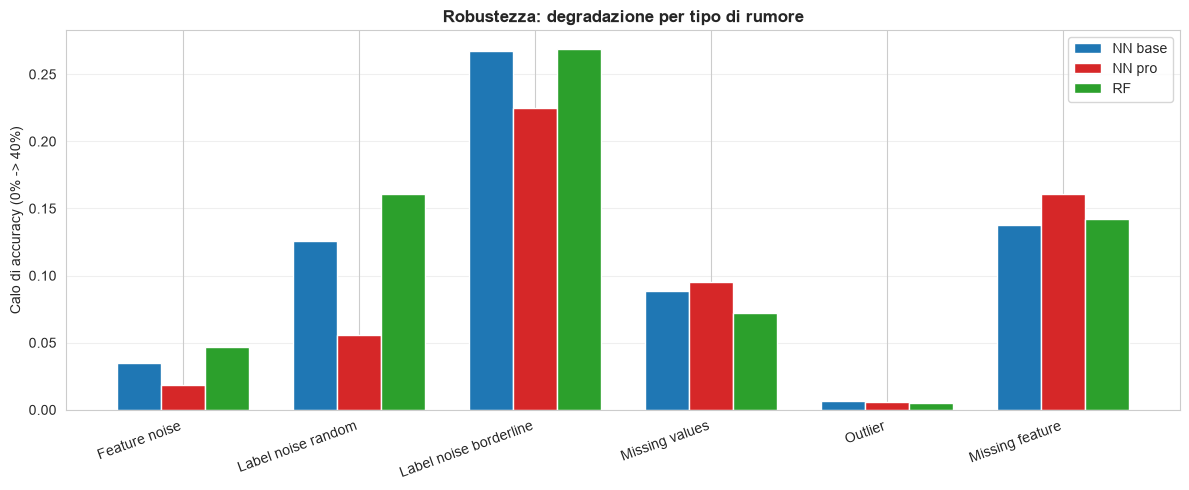
\includegraphics[width=\linewidth]{summary_degradation}\\
      {\scriptsize Barre piccole $=$ maggiore tenuta al rumore.}
    \end{column}
    \begin{column}{0.42\textwidth}
      \centering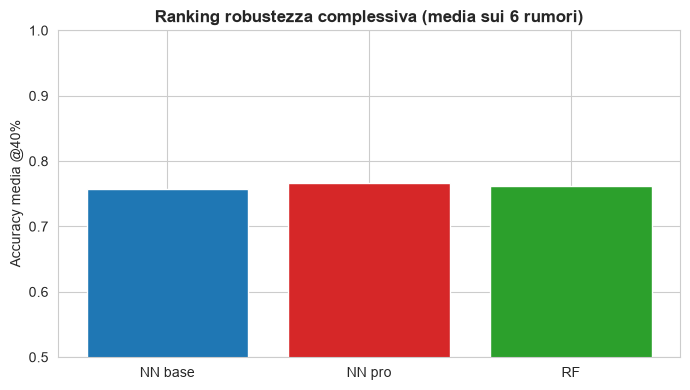
\includegraphics[width=0.92\linewidth]{summary_ranking}\\
      {\scriptsize Robustezza media (caso peggiore).}
      \vspace{0.2cm}
      \begin{itemize}
        \item NN Pro $0{,}785$
        \item RF $0{,}780$
        \item NN Base $0{,}778$
      \end{itemize}
      {\scriptsize Distanze trascurabili: \textbf{nessun vincitore netto}.}
    \end{column}
  \end{columns}
\end{frame}

\begin{frame}{Chi vince su cosa}
  \centering
  \footnotesize
  \begin{tabular}{lll}
    \toprule
    \textbf{Scenario} & \textbf{Modello più robusto} & \textbf{Nota} \\
    \midrule
    Dati puliti        & Random Forest & migliore su tutte le metriche \\
    Feature noise      & NN Pro        & L2 $+$ dropout filtrano il rumore \\
    Label noise random & NN Pro        & early stopping blocca la memorizzazione \\
    Missing values     & Random Forest & opera per divisioni \\
    Outlier            & tutti (pari)  & disturbo quasi innocuo \\
    Missing feature    & Random Forest & NN Pro la \emph{meno} robusta \\
    Label borderline   & nessuno       & collasso generale ($\sim 60\%$) \\
    \bottomrule
  \end{tabular}
  \keypoint{La scelta del modello dipende dal \textbf{tipo di errore atteso} nel
  dominio applicativo, non da una superiorità astratta.}
\end{frame}

\begin{frame}{Curve ROC: il ranking resiste al feature noise}
  \begin{columns}[c]
    \begin{column}{0.6\textwidth}
      \centering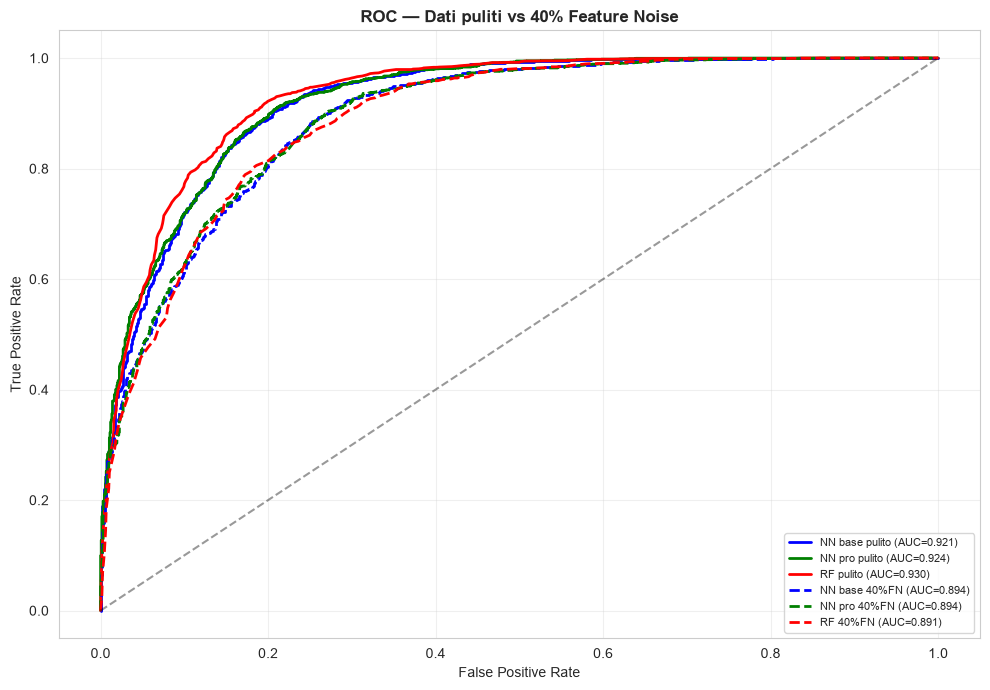
\includegraphics[width=\linewidth]{roc_clean_vs_fn40}
    \end{column}
    \begin{column}{0.4\textwidth}
      \begin{itemize}
        \item Continue $=$ dati puliti; tratteggiate $=$ $40\%$ feature noise.
        \item Lo scarto è limitato: il \textbf{potere di ranking} si riduce poco.
        \item Conferma che il feature noise degrada soprattutto la decisione a
              soglia fissa, non l'ordinamento probabilistico.
      \end{itemize}
    \end{column}
  \end{columns}
\end{frame}

% ============================================================
\section{Analisi non supervisionata (K-Means)}
% ============================================================
\begin{frame}{K-Means: perché e come}
  \begin{columns}[c]
    \begin{column}{0.55\textwidth}
      \centering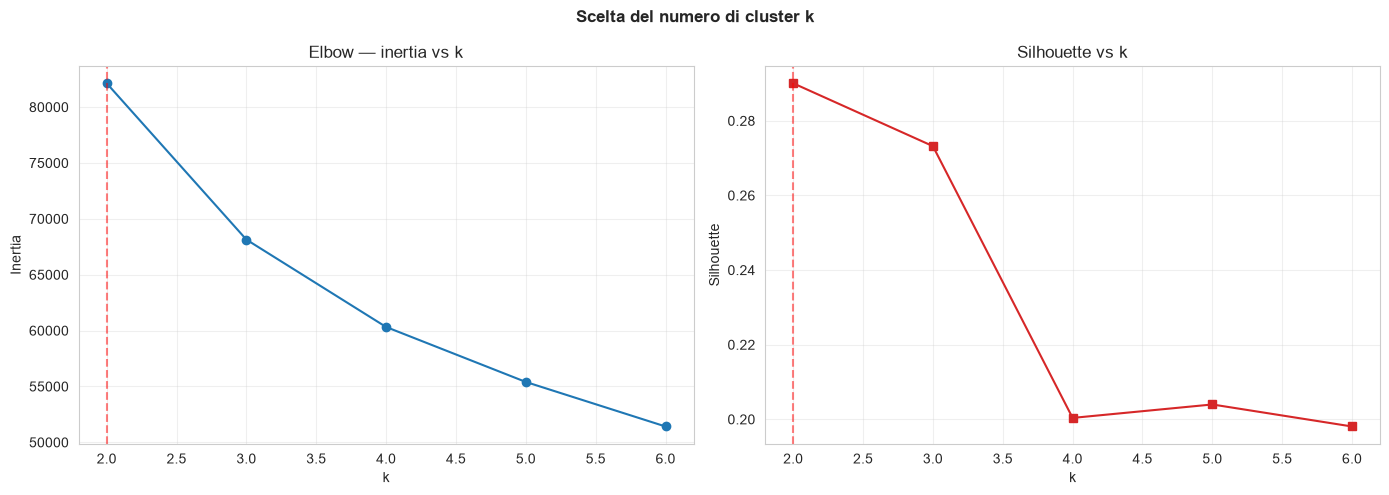
\includegraphics[width=\linewidth]{kmeans_kselection}
    \end{column}
    \begin{column}{0.45\textwidth}
      \begin{itemize}
        \item Esperimento \textbf{senza etichette}: cosa trova un algoritmo basato
              solo sulla distanza?
        \item $k=2$ scelto con \emph{elbow} (inerzia) e \emph{silhouette}
              (massima in $k=2$).
        \item La silhouette tende a premiare $k$ piccoli: indizio, non prova.
      \end{itemize}
    \end{column}
  \end{columns}
\end{frame}

\begin{frame}{K-Means: i cluster non sono le classi}
  \begin{columns}[c]
    \begin{column}{0.6\textwidth}
      \centering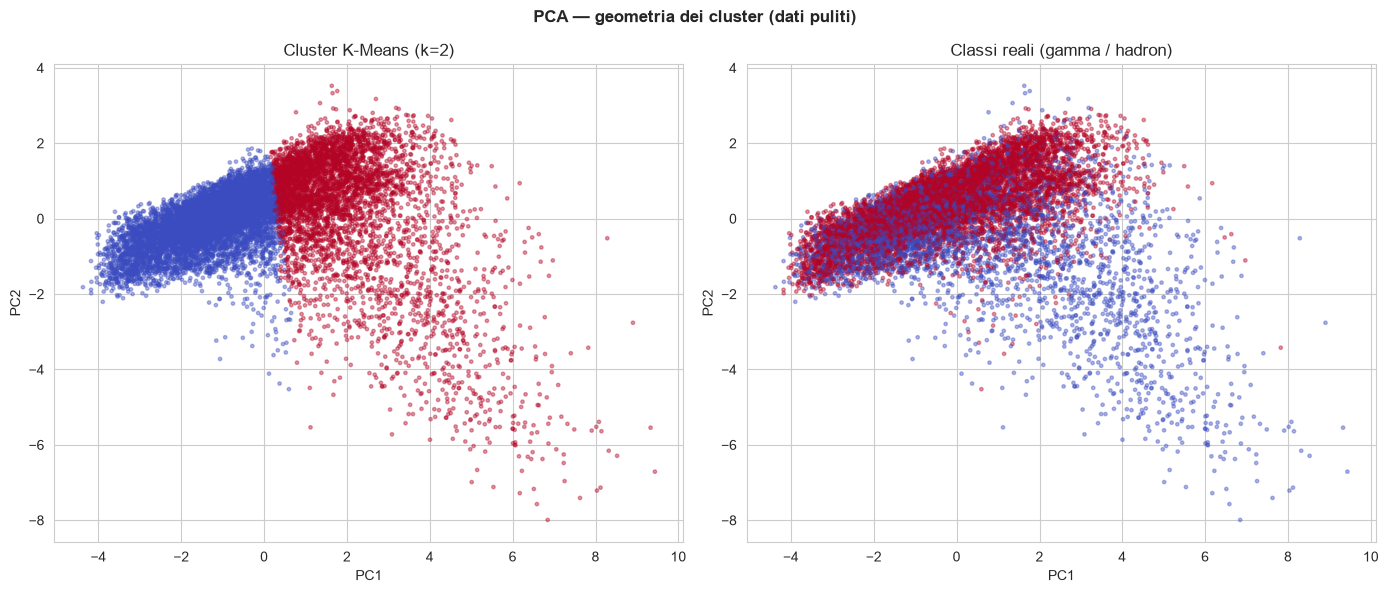
\includegraphics[width=\linewidth]{kmeans_pca}
    \end{column}
    \begin{column}{0.4\textwidth}
      \begin{itemize}
        \item \textbf{ARI $\approx 0{,}006$}, purezza $\approx 0{,}648$ (pari allo
              sbilanciamento nativo).
        \item I cluster dividono lo spazio lungo la \textbf{varianza dominante},
              non la separazione fisica gamma/adrone.
        \item Le proprietà che distinguono le classi attraversano i cluster: nessun
              discriminante lineare.
      \end{itemize}
    \end{column}
  \end{columns}
\end{frame}

\begin{frame}{K-Means sotto rumore}
  \begin{columns}[c]
    \begin{column}{0.5\textwidth}
      \centering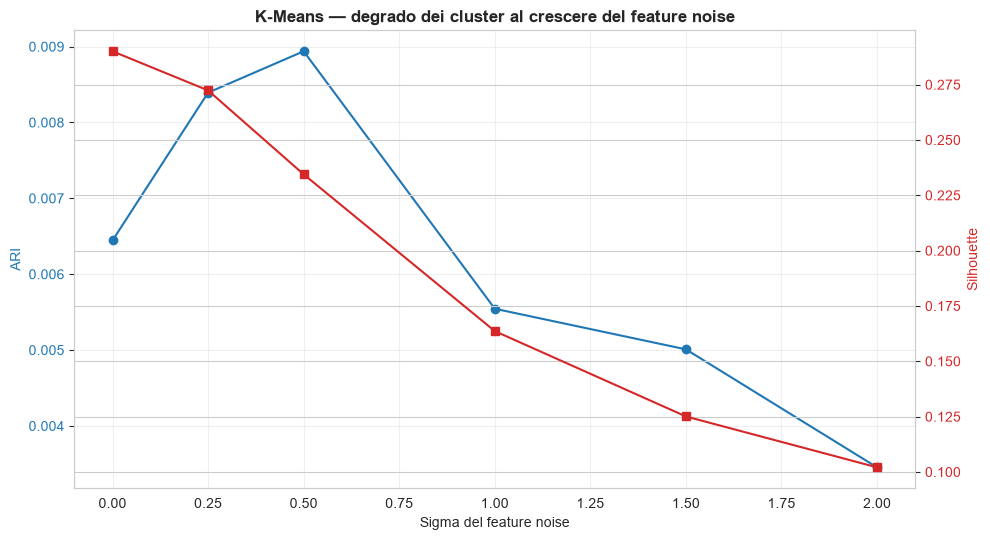
\includegraphics[width=\linewidth]{kmeans_noise}\\
      {\scriptsize ARI e silhouette al crescere del rumore.}
    \end{column}
    \begin{column}{0.5\textwidth}
      \centering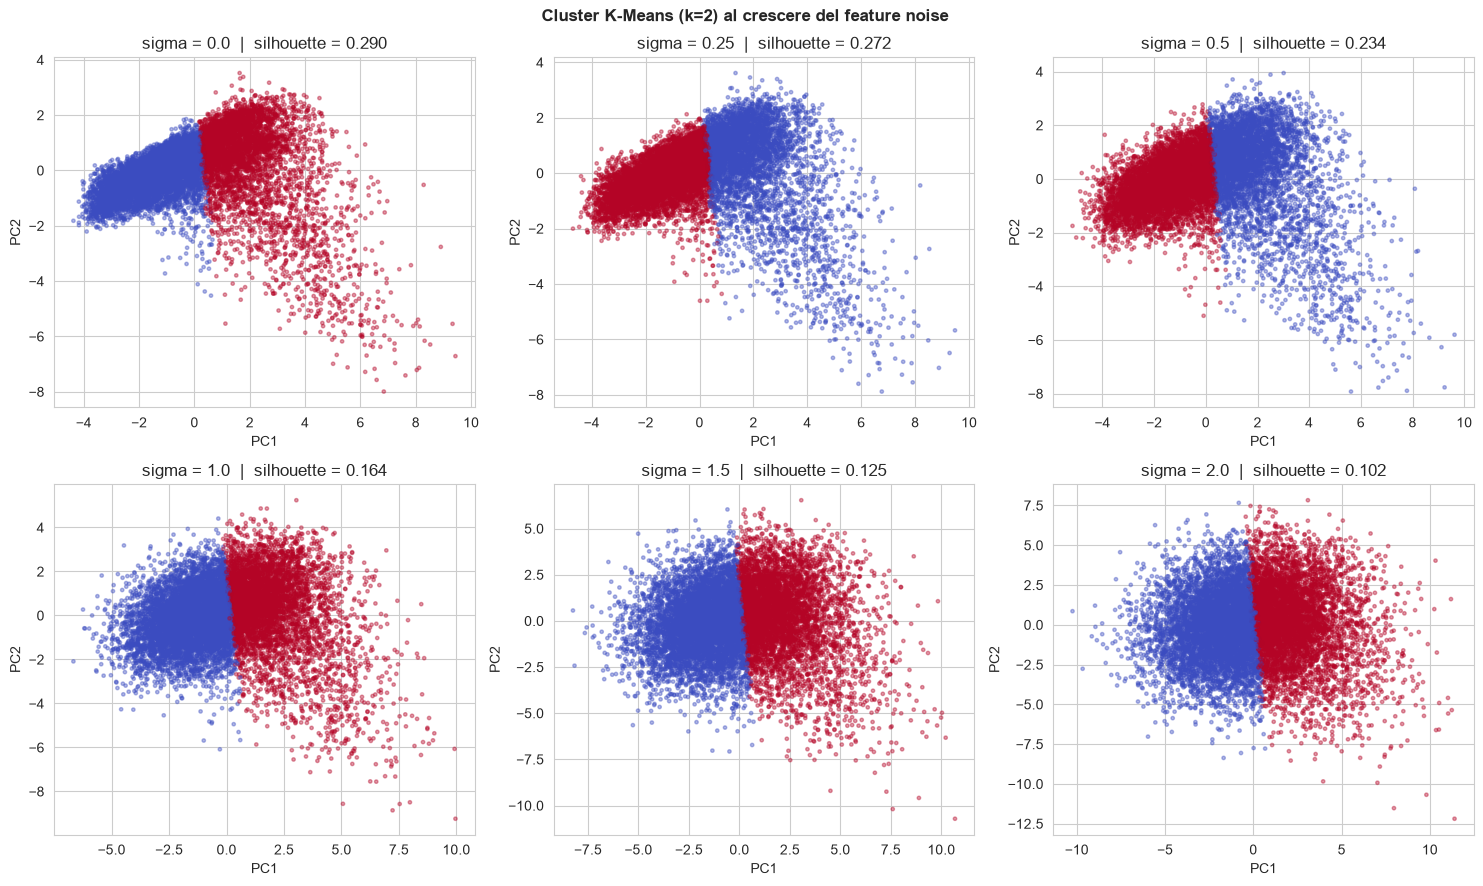
\includegraphics[width=\linewidth]{kmeans_noise_pca}\\
      {\scriptsize I confini dei cluster diventano meno netti all'aumentare di $\sigma$.}
    \end{column}
  \end{columns}
  \vspace{0.1cm}
  \keypoint{Il \textbf{feature noise} degrada i cluster (silhouette
  $0{,}290 \to 0{,}102$). Il \textbf{label noise} non ha alcun effetto
  (ARI $=1{,}000$): K-Means non usa le etichette.}
\end{frame}

\begin{frame}{K-Means: la lezione trasversale}
  \begin{itemize}
    \item La vulnerabilità a un rumore dipende strettamente dalle
          \textbf{informazioni che il modello sfrutta}.
    \item Il label noise -- devastante per i modelli supervisionati -- è
          \textbf{del tutto ininfluente} per K-Means, che ignora le etichette.
    \item Il feature noise -- gestibile nel supervisionato grazie alla ridondanza
          -- \textbf{degrada} la struttura geometrica su cui K-Means si fonda.
  \end{itemize}
  \vfill
  \keypoint{Ciò che è critico per un task può essere irrilevante per un altro:
  la robustezza è sempre \textbf{relativa al modo in cui si usano i dati}.}
\end{frame}

% ============================================================
\section{Conclusioni}
% ============================================================
\begin{frame}{Conclusioni -- i rumori}
  \begin{itemize}
    \item Esiste una chiara \textbf{gerarchia di pericolosità}:
          \begin{itemize}
            \item[$\circ$] \emph{trascurabili}: outlier;
            \item[$\circ$] \emph{gestibili}: feature noise, missing values
                  (ridondanza e imputazione);
            \item[$\circ$] \emph{critici}: missing feature e label noise.
          \end{itemize}
    \item Missing feature e label noise sono gravi per ragioni \textbf{opposte}:
          il primo cancella informazione insostituibile, il secondo forza a
          memorizzare pattern errati.
    \item Il caso peggiore è il \textbf{label noise borderline}: falsifica
          direttamente il confine decisionale.
    \item Il degrado è spesso \textbf{asimmetrico}: a peggiorare è la classe
          minoritaria (adroni); il class weight della NN Pro la protegge.
  \end{itemize}
\end{frame}

\begin{frame}{Conclusioni -- i modelli e il preprocessing}
  \begin{itemize}
    \item \textbf{Nessun modello domina}: la NN Pro vince sul rumore delle
          etichette, il Random Forest su valori mancanti e outlier, la NN Base è
          la più esposta.
    \item La scelta del modello richiede un'analisi \emph{a priori} sui tipi di
          errore attesi nel dominio reale.
    \item L'evidenza più forte: conta \textbf{più il preprocessing} della
          complessità algoritmica.
          \begin{itemize}
            \item[$\circ$] imputazione, winsorizzazione, early stopping recuperano
                  gran parte del degrado.
          \end{itemize}
    \item Ma nessun modello recupera un'informazione \textbf{cancellata} o
          \textbf{falsificata} nei punti più sensibili.
  \end{itemize}
  \vfill
  \keypoint{La robustezza si costruisce a monte (cura del dato) tanto quanto a
  valle (scelta dell'algoritmo).}
\end{frame}

\begin{frame}{Limiti e sviluppi futuri}
  \begin{itemize}
    \item Il controllo multi-seed copre solo il feature noise: va esteso agli
          altri disturbi, in particolare al label noise.
    \item Soglia di decisione fissa a $0{,}5$: ritararla sul validation set
          potrebbe recuperare parte della recall sugli adroni.
    \item Iperparametri scelti sui dati puliti e mai ricalibrati sotto rumore.
    \item Alberi del Random Forest senza limite di profondità: limitarla
          dovrebbe ridurre la memorizzazione delle etichette invertite.
    \item Un solo dataset: la gerarchia osservata dipende anche dalla ridondanza
          tra le feature e dal ruolo di \feat{fAlpha}; va confermata su dataset
          con struttura diversa.
  \end{itemize}
\end{frame}

\begin{frame}[plain]
  \centering
  \vfill
  {\Large Grazie per l'attenzione}
  \vfill
  {\small Daniele Maccagnan \quad Matias Bonoli \quad Ashley Chudory}
  \vfill
  {\footnotesize Studio di robustezza al rumore -- MAGIC Gamma Telescope}
  \vfill
\end{frame}

\end{document}
